\documentclass{sig-alternate}

\usepackage{graphicx}
\usepackage{caption}
\usepackage{subcaption}

\begin{document}
%
% --- Author Metadata here ---
\conferenceinfo{WOODSTOCK}{'97 El Paso, Texas USA}
%\CopyrightYear{2012} % Allows default copyright year (20XX) to be over-ridden - IF NEED BE.
%\crdata{0-12345-67-8/90/01}  % Allows default copyright data (0-89791-88-6/97/05) to be over-ridden - IF NEED BE.
% --- End of Author Metadata ---

\title{Cartographic documents for web modeling of indoor mapping with interactive environments}
\subtitle{[Extended Abstract]
\titlenote{A full version of this paper is available as
\emph{Author's Guide to Preparing ACM SIG Proceedings Using
\LaTeX$2_\epsilon$\ and BibTeX} at
\texttt{www.acm.org/eaddress.htm}}}
%
% You need the command \numberofauthors to handle the 'placement
% and alignment' of the authors beneath the title.
%
% For aesthetic reasons, we recommend 'three authors at a time'
% i.e. three 'name/affiliation blocks' be placed beneath the title.
%
% NOTE: You are NOT restricted in how many 'rows' of
% "name/affiliations" may appear. We just ask that you restrict
% the number of 'columns' to three.
%
% Because of the available 'opening page real-estate'
% we ask you to refrain from putting more than six authors
% (two rows with three columns) beneath the article title.
% More than six makes the first-page appear very cluttered indeed.
%
% Use the \alignauthor commands to handle the names
% and affiliations for an 'aesthetic maximum' of six authors.
% Add names, affiliations, addresses for
% the seventh etc. author(s) as the argument for the
% \additionalauthors command.
% These 'additional authors' will be output/set for you
% without further effort on your part as the last section in
% the body of your article BEFORE References or any Appendices.

\numberofauthors{6}
\author{
% You can go ahead and credit any number of authors here,
% e.g. one 'row of three' or two rows (consisting of one row of three
% and a second row of one, two or three).
%
% The command \alignauthor (no curly braces needed) should
% precede each author name, affiliation/snail-mail address and
% e-mail address. Additionally, tag each line of
% affiliation/address with \affaddr, and tag the
% e-mail address with \email.
%
\alignauthor
Marco Virgadamo\\
       \affaddr{Dipartimento di Ingegneria}\\
       \affaddr{Universit\`a Roma Tre}\\
       \affaddr{Rome, Italy}\\
       \email{dvr@dia.uniroma3.it}
\alignauthor
Marco Sportillo\\
       \affaddr{Dipartimento di Ingegneria}\\
       \affaddr{Universit\`a Roma Tre}\\
       \affaddr{Rome, Italy}\\
       \email{dvr@dia.uniroma3.it}
\alignauthor 
Federico Spini\\
       \affaddr{Dipartimento di Ingegneria}\\
       \affaddr{Universit\`a Roma Tre}\\
       \affaddr{Rome, Italy}\\
       \email{dvr@dia.uniroma3.it}
\and  % use '\and' if you need 'another row' of author names
\alignauthor 
Alberto Paoluzzi\\
       \affaddr{Dip. di Matematica e Fisica}\\
       \affaddr{Universit\`a Roma Tre}\\
       \affaddr{Rome, Italy}\\
       \email{dvr@dia.uniroma3.it}
\alignauthor 
Enrico Marino\\
       \affaddr{Dipartimento di Ingegneria}\\
       \affaddr{Universit\`a Roma Tre}\\
       \affaddr{Rome, Italy}\\
       \email{dvr@dia.uniroma3.it}
\alignauthor 
Antonio Bottaro\\
       \affaddr{SOGEI S.p.a.}\\
       \affaddr{Ricerca e Sviluppo}\\
       \affaddr{Rome, Italy}\\
       \email{dvr@dia.uniroma3.it}
}

\maketitle \begin{abstract} This paper introduces the HIJSON, a novel indoor
cartographical document format. A software framework is also presented, that
relies on HIJSON documents and is entirely based on web technologies. With
respect to current cartographic formats, the HIJSON brings three major
enhancements: it exposes a hierarchical structure, uses metric local
coordinate system and accepts semantic extensions. HIJSON format is designed
to homogeneously describe both the geometry of an indoor space, capturing its
complete topology, and all the objects (smart or not) contained in it. Such a
representation allows the software framework to offer a web environment in
which the user is presented with both 2D and 3D models of the indoor ambience.
This virtually rebuilt environment, accessible via web browsers from any kind
of device, represents the platform in which several applications can coexist:
IoT monitoring, realtime multi-person tracking, crossfloor user navigation, 
through an algorithm that automatically finds a valid walkable routes for 
indoor einvonments, taking into account both architectural encumbrances and furniture.
Semantic extensions provided by HIJSON and supported by the
detailed framework architecture encapsulate details about communication
protocols, exchanged and displayed information, allowing the HIJSON format to
be extened with any kind of objects, sensors or behaviors. \end{abstract}

% A category with the (minimum) three required fields
\category{H.4}{Information Systems Applications}{Miscellaneous}
%A category including the fourth, optional field follows...
\category{D.2.8}{Software Engineering}{Metrics}[complexity measures, performance measures]

\terms{Theory}

\keywords{indoor cartography, indoor navigation, IoT monitoring, multiperson-tracking}

\section{Introduction}\label{introduction}

CARATTERISTICHE E SPUNTI:

\begin{itemize}
\item
  CONNESSIONE CON I SENSORI PER LA RILEVAZIONE DELLA POSIZIONE DEI
  VISITATORI
\item
\item
\end{itemize}

\ldots{}

The remainder of this document is organized as follows. In Section II is
provided an overview of the state of the art. Section III is devoted to
describe the novel cartographic document proposed, while section IV introduces
the underlying mathematical structure. Section V reports about the tools and
instruments developed specifically for the web, focusing on software
architecture, implemented algorithms and real applications. Section VI
describes one use case of both document format and software tools. Finally
Section VII proposes some conclusive remarks and future developments.

\section{State of the art}\label{state-of-the-art}

Researches about the cartographic representation of indoor environments are
numerous and at the same time heterogeneos regarding to the strategies
applied. Different sources of information are used and accuracy of the
produced solution depends on the adopted approach. In some cases the
information  is obtained with automatic or semi-automatic processing of files
that describe the  architectural structure of a building, such as BIM (Link a
BIM) and/or IFC (Link a IFC) \cite{6816739}. Image processing is also used to
extract topological information from floor plan images \cite{6878152}. In
other works, building informations and descriptive parameters are redefined
from scratch \cite{6418876}.  This choice is driven by the unsuitableness of
the current representive formats:  images contain poor information and CAD
files are not designed for this kind of use. A recurring topic among the use
of carthograhic information is indoor navigation
\cite{6878152,6418876,6816739}. The proposed approaches are very different in
this case too, and based on several strategies with some basic elements in
common. An often adopted solution is based on the representation of the
routing information as a graph, having a node for each room and an edge for
each couple of connected rooms. In some cases the edges are weighted in
function of euclidean distance. The detail level of the graph and hence the
effective practicalbility of the calculated paths, can vary depending on the
technique and the design choices applied, but in general most of the proposed
solutions retrieve information only from architectual structure. A topic
related to the navigation is the location of users. All the considered works
agree on the inadequacy of GNSS in indoors contexts, due to the segnificant
reduction in signal quality. To locate the exact position of a user inside a
building, the currently most used techniques are based on fingerprinting and
triangulation of radio signals (WiFi, Bluetooth, etc.) flanked by more
original solutions based on, for example, image recognition \cite{6815564}.
User tracking issue is faced with solutions that range from the clever
utilization of inertial tracking sensors embedded in many smartphones
\cite{6815564} to the adoption of ad hoc devices \cite{6878152}.

The actual ``de-facto'' standard in terms of geospatial data representation is
the GeoJSON format, which can be easily used for any type of geographical
annotation. In some cases it has been slightly adapted to be used in indoor
environments (IndoorJSON).

\subsection{The GeoJSON format}\label{the-geojson-format}

GeoJSON is a geospatial data interchange format based on JSON, suitable for a
geometrical encoding of various geographic data structures. As opposed to GIS
format, GeoJSON is an open standard. Positions need to be expressed in
geographical coordinates (usually WGS84).

GeoJSON supports the following geometry primitives: \texttt{Point},
\texttt{LineString}, \texttt{Polygon}, \texttt{MultiPoint},
\texttt{MultiLineString}, and \texttt{MultiPolygon}. Lists of geometries are
represented by a \texttt{GeometryCollection}. Geometries with additional
properties are \texttt{Feature} objects. Lists of \texttt{Feature} are
represented by a \texttt{FeatureCollection}.

A single \texttt{Feature} is composed essentially by two mandatory fields:
\texttt{geometry}, which describes the objects' geometry accordingly to the
previously defined primitives, and \texttt{properties} which contains
additional  information about the \texttt{Feature}.

It is possible to define complex shapes through the composition of simple
GeoJSON objects. Mainly due to its semplicity, GeoJSON is widely used and
deeply integrated in several applications and services.

\subsection{The IndoorJSON format}\label{experiences-on-indoor-json}

IndoorJSON is a GeoJSON variant defined and used by \emph{indoor.io}, a
Finnish company devoted to indoor environment mapping. IndoorJSON is compliant
with GeoJSON syntax, and it may consist of any number of \texttt{Features}
and/or \texttt{FeatureCollections}. All \texttt{Features} are interpreted
similarly regardless of their grouping into nested
\texttt{FeatureCollections}. IndoorJSON supports all GeoJSON geometry types.

Some particular properties are used to correctly define indoor elements:

\begin{itemize}
\itemsep1pt\parskip0pt\parsep0pt
\item
  \texttt{level}: described which level contains the feature;
\item
  \texttt{geomType}: identifies the object's
  category, useful during the visualization
  process.
\end{itemize}

There are some additional not mandatories properties useful for
the indoor representation:

\begin{itemize}
\itemsep1pt\parskip0pt\parsep0pt
\item
  \texttt{accessible}: describes if an element is walkable or not;
\item
  \texttt{connector}: defines if the element is a connection between two
  levels;
\item
  \texttt{direction}: describes the direction of the connection (both
  ways, only up, only down);
\end{itemize}

A syntax validator is provided by \emph{indoor.io}, but the commercial nature
of  this project limits the number of tools available to deal with this
format.

\section{Advances on cartographic document formats}\label{advances-on-cartographic-document-format}

The focus of this work is the definition of a novel format of cartographic
documents along with the software ecosystem rooted on it. A simple but
effective  algorithm to find indoor valid routes is also provided. The
\textbf{HIJSON} (\textbf{H}ierarchical \textbf{I}ndoor \textbf{JSON}, this is
the name chosen for the format) and the accompanying software framework aim
to realize a mapping of indoor real spaces with a virtual interactive web
environment. The HIJSON is based upon ideas and design principles collected
from previous formats and identifies three critical improvements with respect
to them: it exposes a \emph{hierarchical structure}, uses \emph{metric local
coordinate system} and accepts \emph{semantic extensions}. Furthermore, geometrical 
and topological data are conveniently imported and represented via LAR, an advanced 
representation scheme, allowing to deal with \emph{hyperlinked geometric models}.

\subsection{Hierarchical structure}\label{hierarchical-structure}

The HIJSON format allows for hierarchical description of indoor spaces.  The
introduction of a hierarchical structure establishes a parent-child relation
between entities of the model, reflecting a container-contained relationship.
This direclty implies a neater representation than the plain linear structure
adopted  by GeoJSON, being a perfect analogy of objects contained (i.e.
placed) into spaces.

In addition, more organized arrangement is allowed by logical (or even
physical)  grouping: concepts like building wings, sections, stories,
departemens, etc. can be  introduced to reflect into the document structure
logical or physical real divisions,  categories or relashionships.

Hierarchical structures are common in computer graphics since they are used as
scenegraphs. This accordance of underlying structures really simplify 3D
render algorithms of HIJSON documented environments.

Furthermore the container-contained relation enables to use local reference system.

\subsection{Metric local coordinate system}\label{metric-local-coordinate-system}

Supported by the hierarchical underlying structure, the HJSON document format allows 
for the use of local coordinate system. This means that the shape of all elements can 
be convenient modelled in local coordinate and than placed in the right position 
with respect to the position of the parent (or container) element applying a 
translation and a rotaction vector.

Another substantial advantage is represented by the adoption of a metric reference, 
consequently simplifying the compilation of the document, however it is, 
manual or aided by software tools.

The HIJSON document format is specially designed to guarantee the user to be routed seamlessly 
from outdoor to indoor and vice versa. Even though indoor geometries are inputted in a metric 
local continuous outdoor-indoor navigation is ensured via the definition of a processing pipeline
detailed in the following.

\subsection{Semantic extensions}\label{semantic-extensions}

Semantic extensions make the HIJSON format extendible and customizable, that is, able to 
adequately respond to any object representation need. To define a semantic extension means to allow the HIJSON document to model an object previously not covered, or even to modify the behaviour of a comprised one. Semantic extensions are to be defined both as HIJSON format syntyax and as HIJSON Toolk source code. In particular it is necessary to define respectively a new HIJSON Element and a new HIJSON Class, as specified below.

\subsection{Hyperlinked geometric models}\label{optional-lar}

A HIJSON document may further import external geometric models --- either of the
buildings itself or the interior furniture or devices --- that are topologically
complete (in the sense of solid
modeling~\cite{Requicha:1980:RRS:356827.356833}) and very compact.  Such
models coming from a source outside the document are acquired by linking JSON
files that contain a Linear Algebraic Representation (LAR) of topology and
geometry, to be expanded for visualization or interaction at any useful level
of detail.

The LAR scheme~\cite{Dicarlo:2014:TNL:2543138.2543294} is characterised by a
very large domain, including architecture, building and
construction~\cite{paoluzziMS:2014}, 2D and 3D engineering meshes, non-
manifold geometric and solid models and meshes, and high-resolution 3D
images~\cite{cadanda:2015}. This scheme uses the set of \emph{Combinatorial
Cellular Complexes} (CCC) as mathematical domain \cite{Basak:2010}, and
various compressed representations of \emph{sparse matrices} \cite{gemmexp} as
codomain.

Since LAR provides a complete representation of the topology of the
represented space, the matrix  $[\partial_d]$ of the boundary operator shall
be used to compute the coordinate representation $[c]$ of the \emph{boundary}
chain of \emph{any subset} $c$ of cells, though \emph{a single} operation of
SpMV multiplication \cite{gemmexp} between the \texttt{CSR} (Compressed Sparse
Row) representation of $[\partial]$ and the \texttt{CSC} (Compressed Sparse
Column) representation of the $[c]$ chain, resulting in very efficient
computations on modern hardware, even mobile.

\begin{figure*}[h!tb]
  \centering
  \begin{subfigure}[b]{0.31\textwidth}
  \centering
    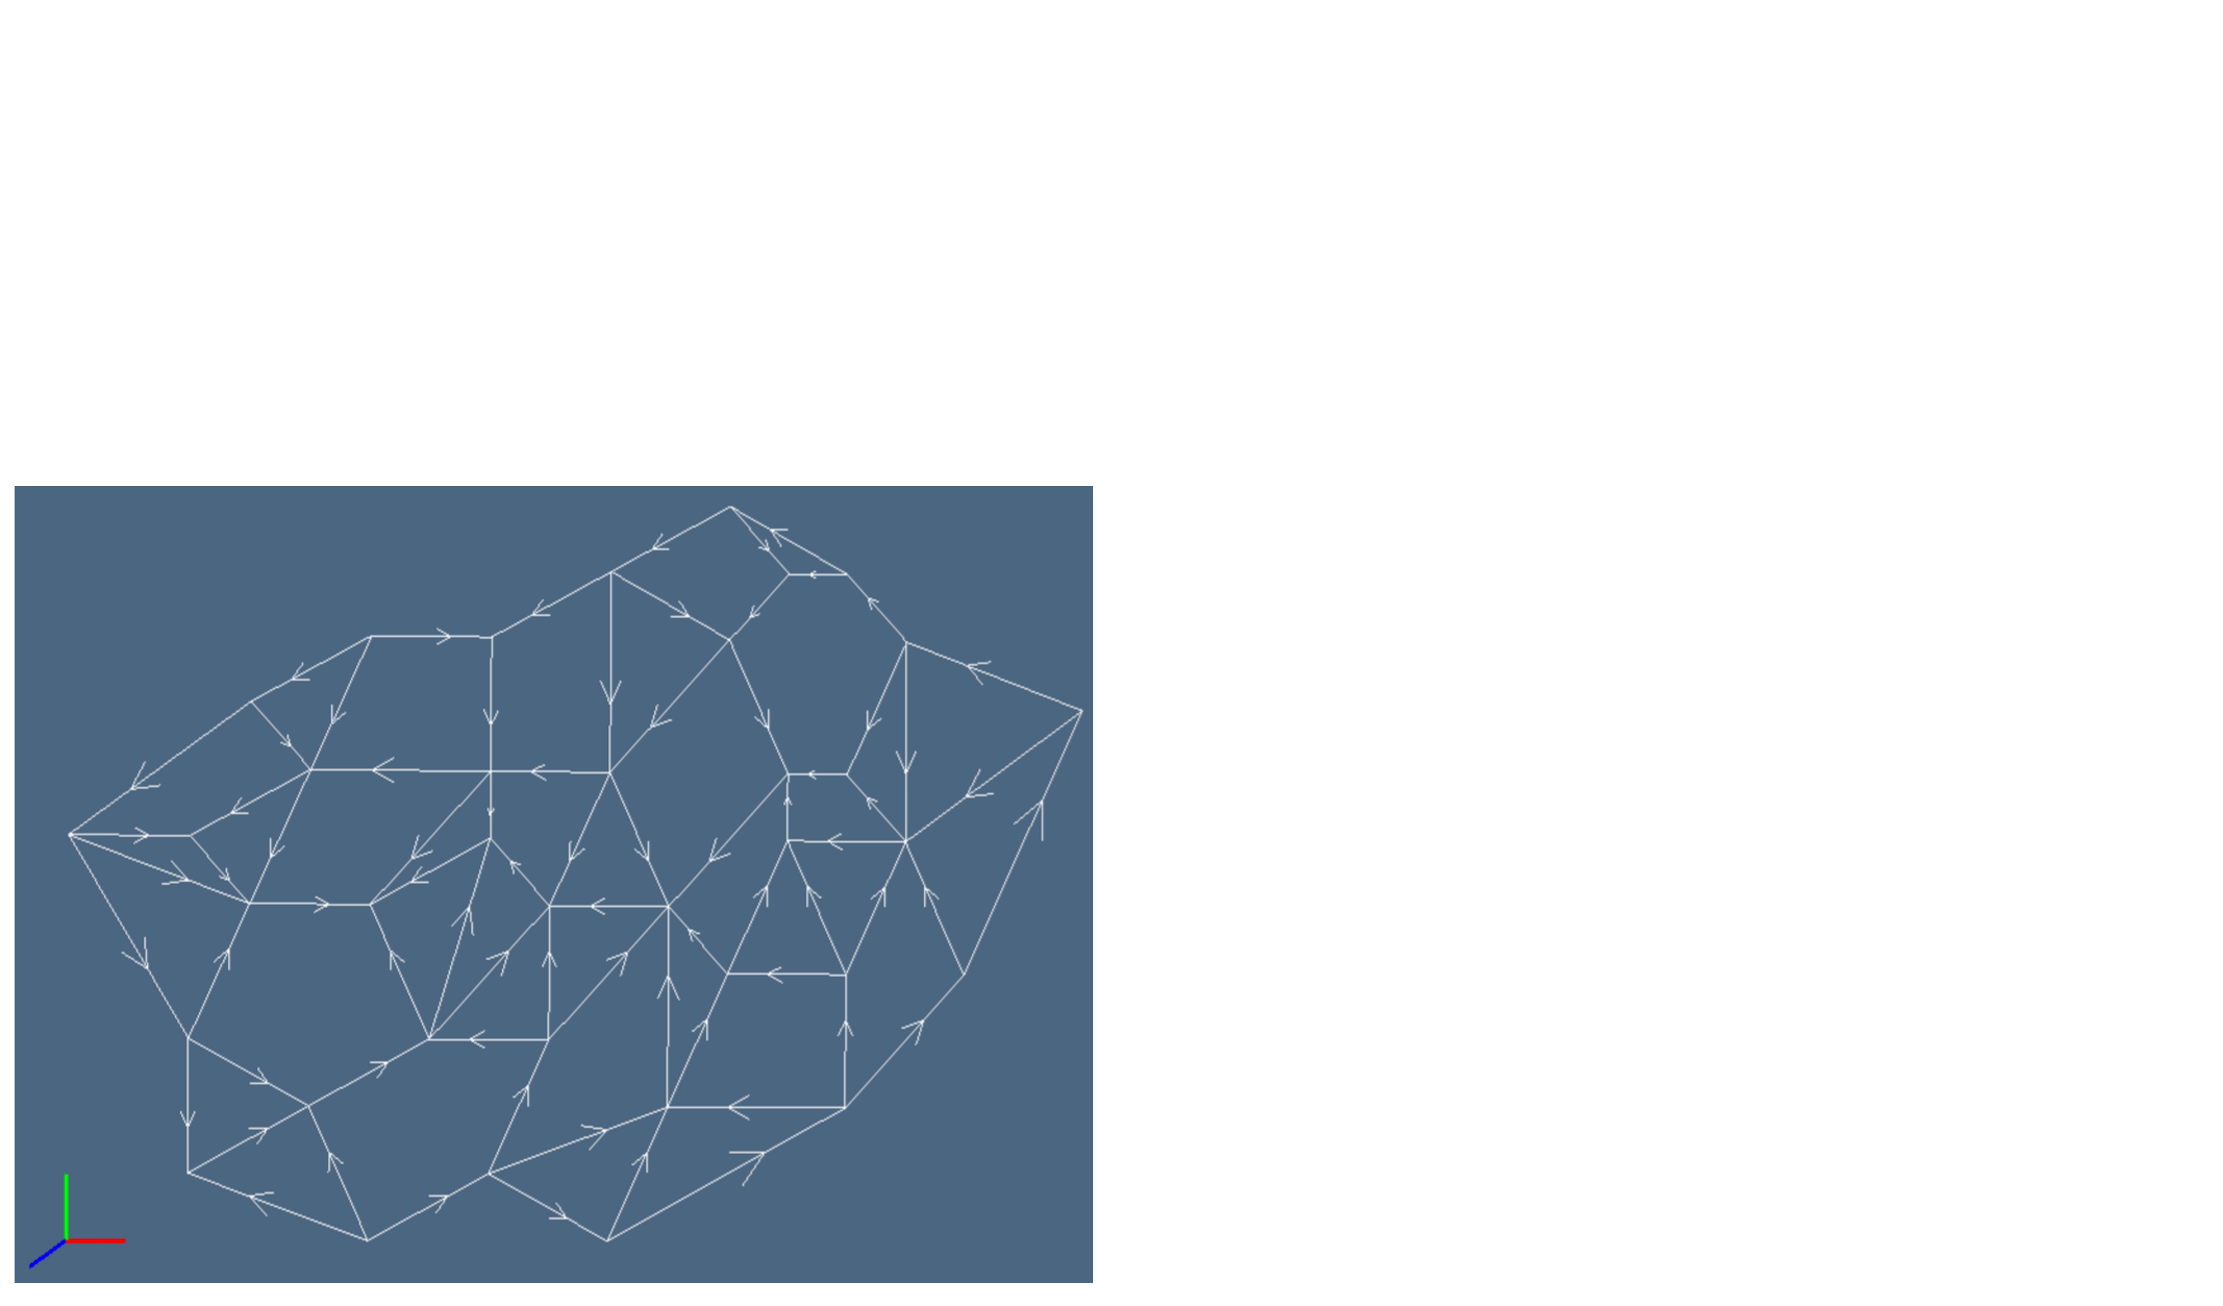
\includegraphics[width=\textwidth]{images/minimum-a} 
    \caption{}
    \label{fig:lar-example-a}
  \end{subfigure}
  ~
  \begin{subfigure}[b]{0.32\textwidth}
  \centering
    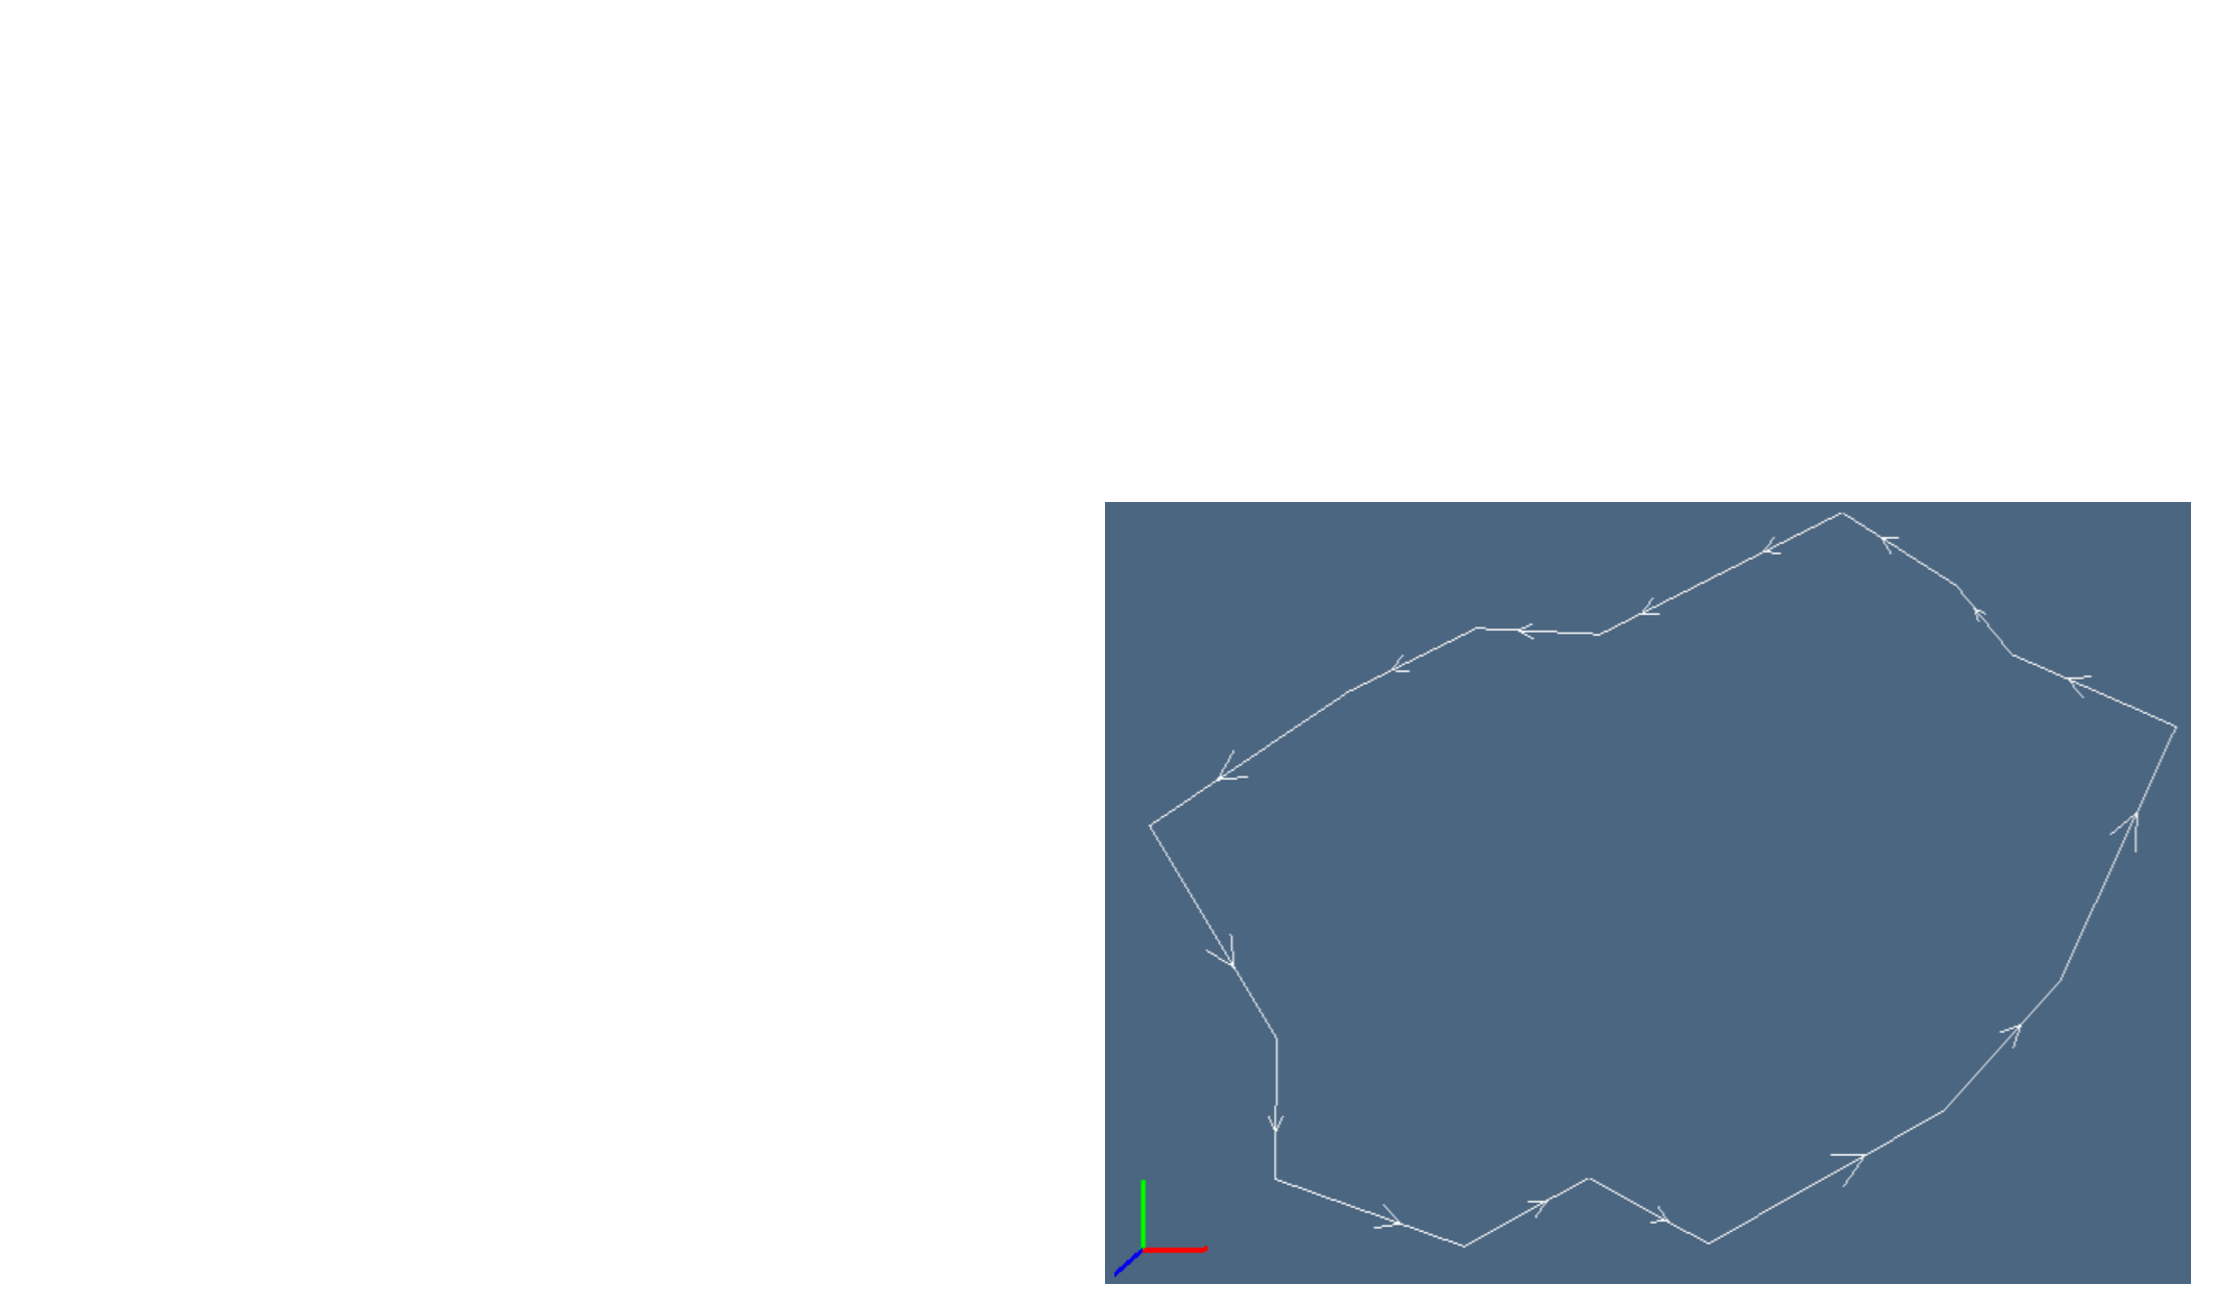
\includegraphics[width=\textwidth]{images/minimum-b} 
    \caption{}
    \label{fig:lar-example-a}
  \end{subfigure}
  ~
  \begin{subfigure}[b]{0.33\textwidth}
    \centering
    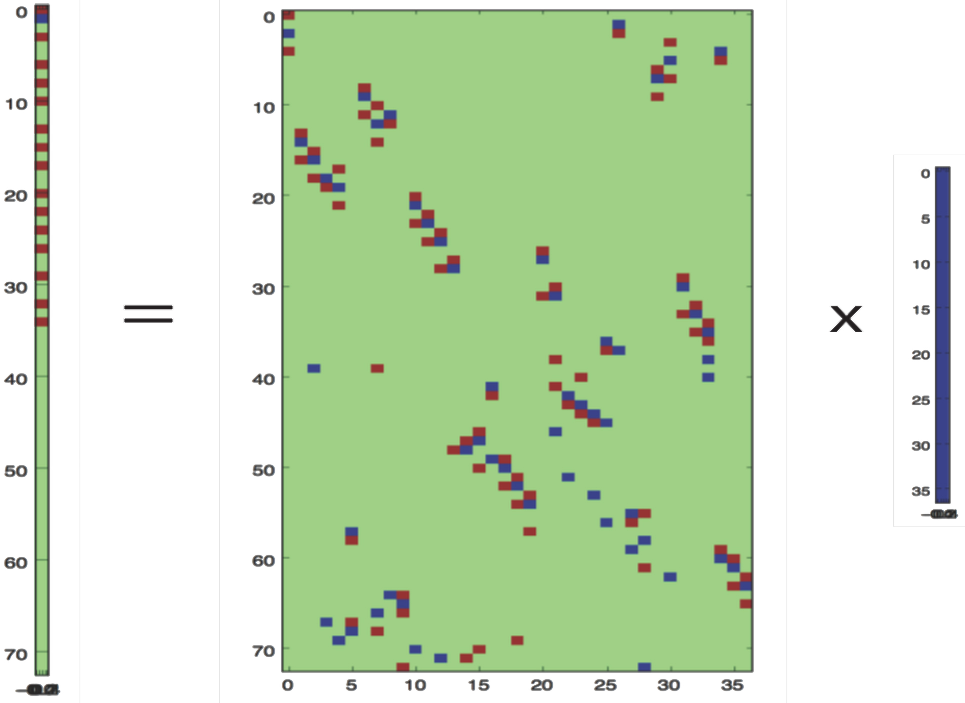
\includegraphics[width=\textwidth]{images/boundary}
    \caption{}
    \label{fig:lar-example-b}
  \end{subfigure}
  
  \caption{A toy example of the LAR scheme: (a) the bare minimum of data with \emph{complete} information about topology: vertices {\scriptsize\texttt{V = [[[5, 0], [[7, 1], [[9, 0], [[13, 2], [[15, 4], [[17, 8], [[14, 9], [[13, 10], [[11, 11], [[9, 10], [[5, 9], [[7, 9], [[3, 8], [[0, 6], [[2, 3], [[2, 1], [[8, 3], [[10, 2], [[13, 4], [[14, 6], [[13, 7], [[12, 10], [[11, 9], [[9, 7], [[7, 7], [[4, 7], [[2, 6], [[3, 5],[[4, 2],[[6, 3],[[11, 4],[[12, 6], [[12, 7], [[10, 5], [[8, 5], [[7, 6], [[5, 5]]}} and faces {\scriptsize\texttt{FV = [[[0, [1, [16, [28, 29], [[0, [15, 28], [[1, [2, 17], [[1, [16, [17, 33], [[2, [3, 17], [[3, [4, [18, 19], [[3, [17, [18, 30], [[4, [5, 19], [[5, [6, 19], [[6, [7, [20, [21, [22, 32], [[6, [19, 20], [[7, [8, 21], [[8, [9, [21, 22], [[9, [11, [23, 24], [[9, [22, 23], [[10, [11, [24, 25], [[10, [12, 25], [[12, [13, [25, 26], [[13, [14, 27], [[13, [26, 27], [[14, [15, 28], [[14, [27, [28, [29, 36], [[16, [29, 34], [[16, [33, 34], [[17, [30, 33], [[18, [19, 31], [[12, [30, 31], [[19, [20, [31, 32], [[22, [23, [32, 33], [[23, [24, [34, 35], [[23, [33, 34], [[24, [25, [27, 36], [[24, [35, 36], [[25, [26, 27], [[29, [34, 35], [[29, [35, 36], [[30, [31, [32, 33]]}}; (b) the extracted boundary; (c) the extraction method $[e] = [\partial][f]$ giving the coordinate representation (in the discrete basis of the 2-cells) ofthe boundary edges $[e]$ by product of the sparse boundary operator matrix $[\partial]$ times the coordinate representation $[f]$ of the 2-cells (faces)}
  \label{fig:minimum}
\end{figure*}

The expansion of a LAR model, to be considered as a general-purpose graphic
primitive, may be executed on either  the server or the supervisor client of
the HIJSON Web Toolkit architecture (see Section~\ref{server-architecture}),
or even on the explorer client, depending on the size and the locality of the
model to be expanded.

\begin{figure}[!h]
  \centering
  \begin{subfigure}[b]{0.48\linewidth}
    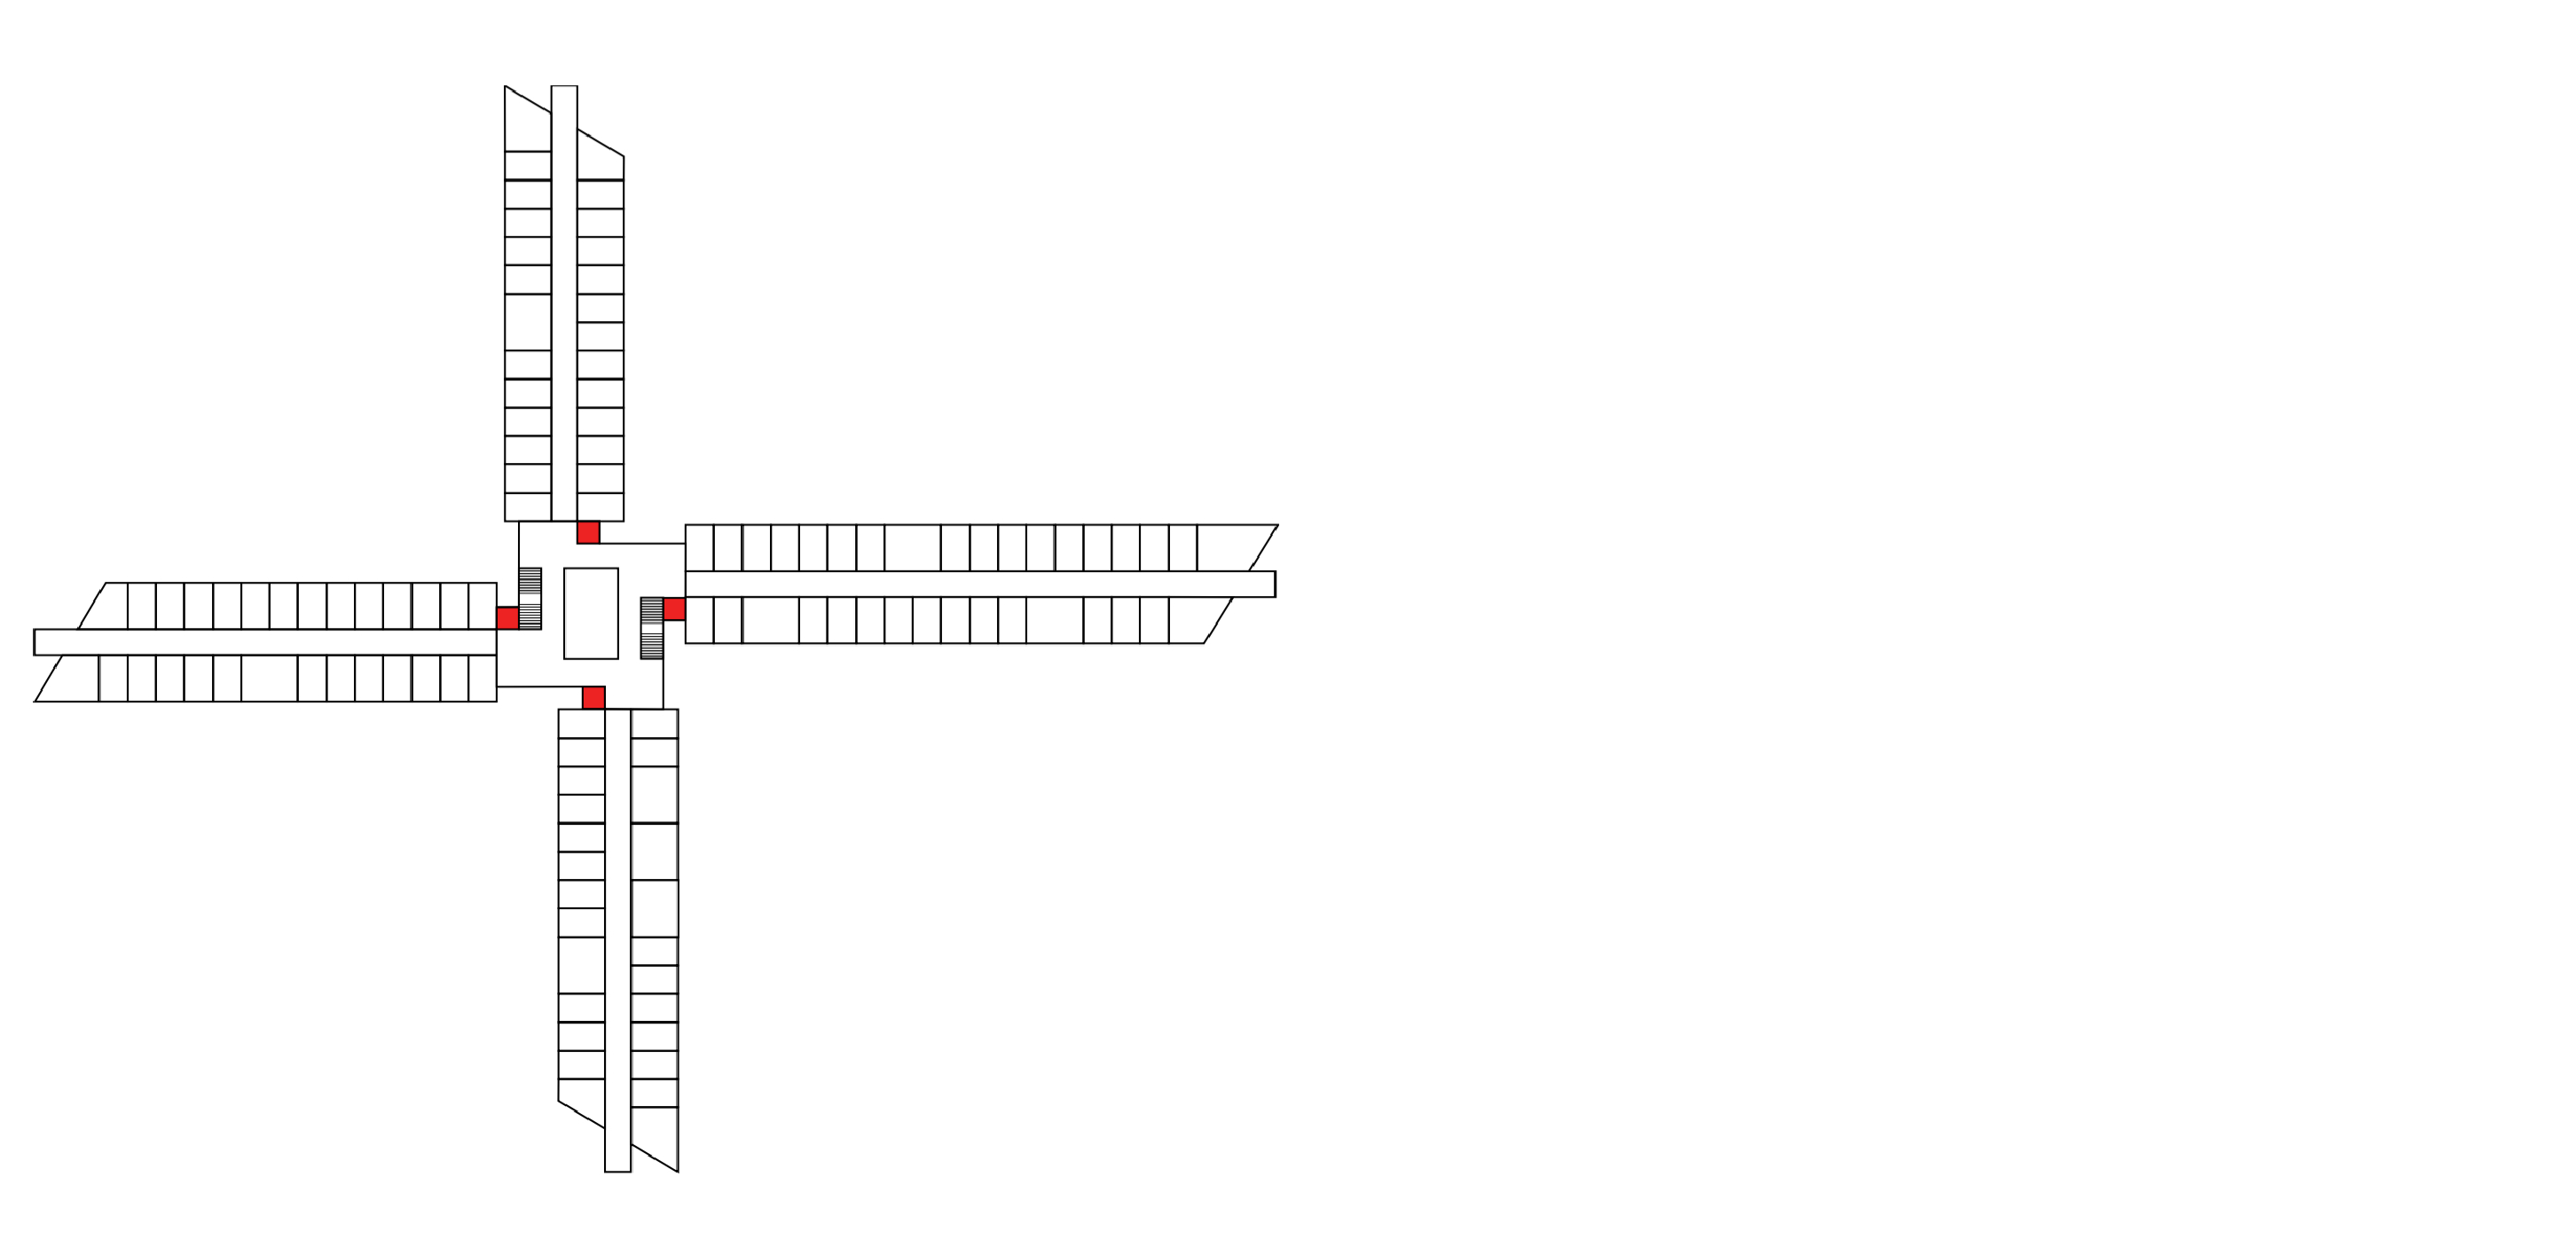
\includegraphics[width=\textwidth]{images/sogei-a} 
    \caption{}
    \label{fig:sogei-a}
  \end{subfigure}
  ~
  \begin{subfigure}[b]{0.48\linewidth}
    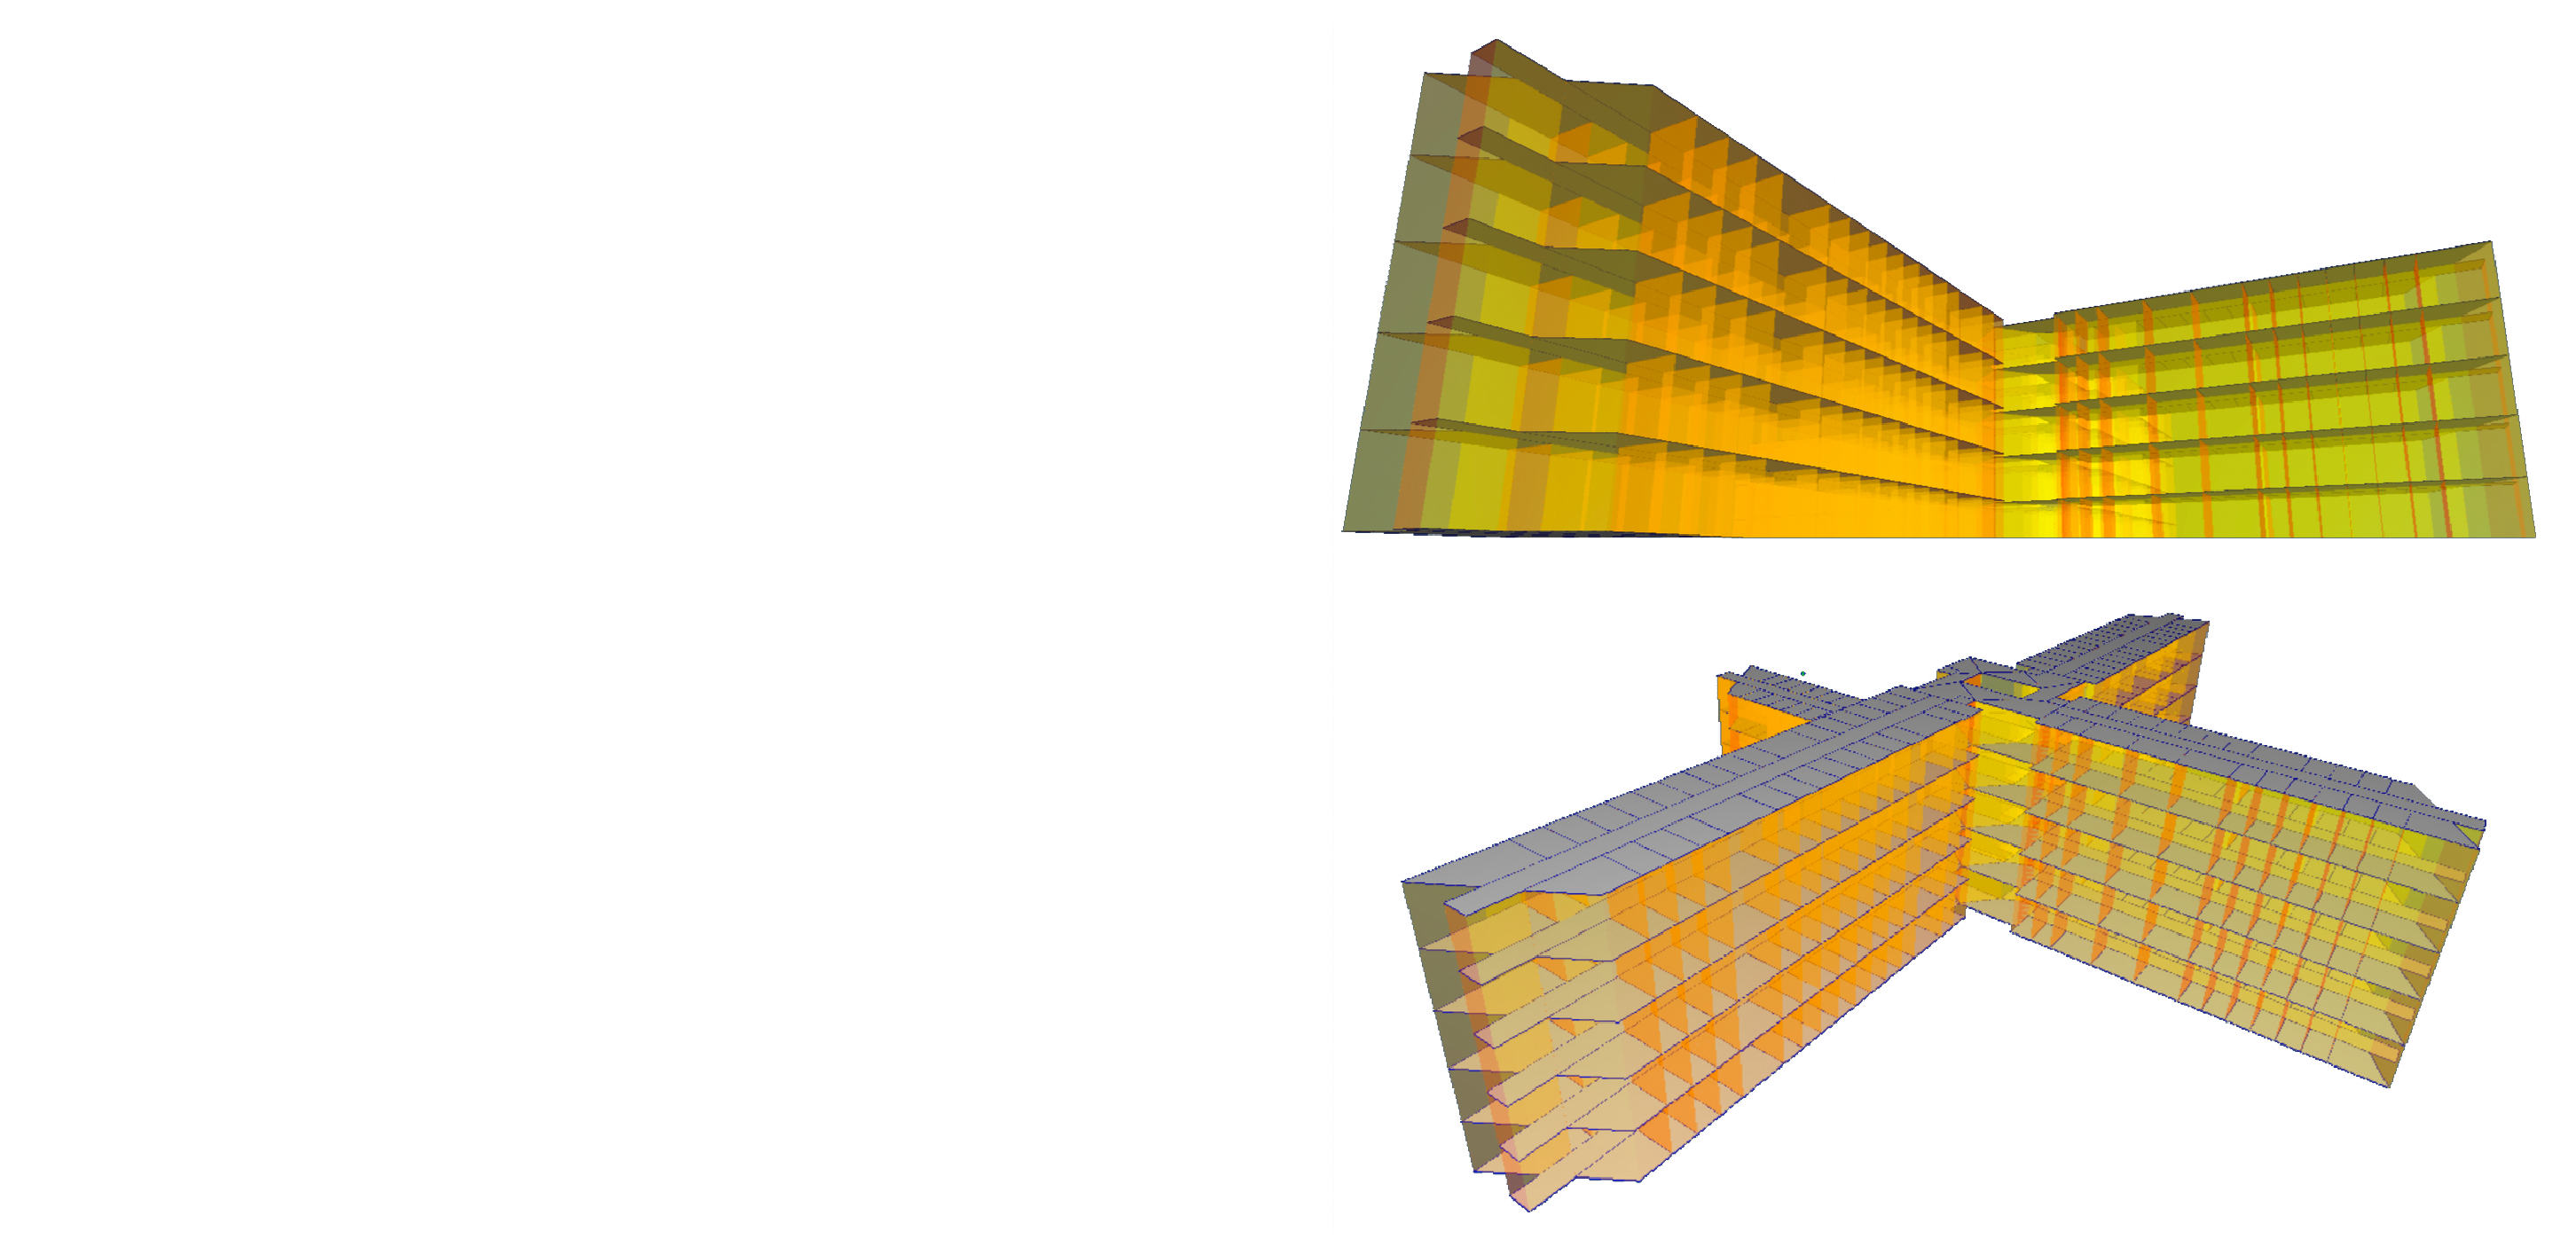
\includegraphics[width=\textwidth]{images/sogei-b}
    \caption{}
    \label{fig:sogei-b}
  \end{subfigure}
  
  \caption{Office building: 
      (a) the schematic plan; 
      (b) the simplified 3D model generated for testing on the field 
        the in-door mapping project described in this paper.
  }
  \label{fig:sogei}
\end{figure}

\section{HIJSON syntax}\label{hijson-syntax}

Below there is an example of an input file ready to be processed by the HIJSON pipeline:

\begin{verbatim}
{
  "config": {
    ...
  },
  "data": 
  [
    ...
    {
      "id": "architecture",
      "type": "FeatureCollection",
      "features": [...] 
    },
    {
      "id": "furniture_1",
      "type": "FeatureCollection",
      "features": [...] 
    },
    ...
  ]
}
\end{verbatim}

The HIJSON document is composed of different parts:

\begin{itemize}
\itemsep1pt\parskip0pt\parsep0pt
\item  
  configuration: a JSON object containing parameters and settings useful
  for the building representation. In particular three points of the local
  reference system are mapped to three couples of geographical coordinates.
  This information allows the computation of the transformation matrix used to
  translate the local coordinates to global ones.
\item
  one or more data collections: each of these lists is given in the form   of
  a GeoJSON FeatureCollection, containing a number of HIJSON   Elements. Since
  HIJSON Elements adhere to the GeoJSON format, each   collection can be
  accepted by a GeoJSON validator. HIJSON introduces   some additional rules
  that allow the adoption of this format for   indoor representation. In the
  next paragraph is given a sample of HIJSON Element, with   the description of
  the main differences from a standard GeoJSON   Feature. 
\end{itemize}

Below there is an example of data collection, with the definition of an HIJSON Element:

\begin{verbatim}
{
  "id": "architecture",
  "type": "FeatureCollection",
  "features": 
  [
    ...
    {
      "type": "Feature",
      "id": "room_0.1",
      "geometry": 
      {
        "type": "Polygon",
        "coordinates": 
        [ 
          [ [0, 0], [11, 0], [11, 19], [0, 19] ]
        ]
      },
      "properties": 
      {
        "class": "room",
        "parent": "level_0",
        "description": "Office of Mr. Smith",
        "tVector": [10, 20, 0],
        "rVector": [0, 0, 90]
    },
    ...
  ]
}
\end{verbatim}

\subsection{HIJSON Element description}

The first additional requisite above the GeoJSON format rules is the
necessity of a unique ID, necessary for the referencing by possible
child elements. The Geometry types allowed are \texttt{Point},
\texttt{LineString} and \texttt{Polygon}. Each geometry type is used to
represent particular categories of elements (e.g.~Polygons for levels
and rooms, LineString for walls and doors, Point for furniture, etc.).
The geometry coordinates are expressed in meters, and for convention
starting at the bottom-left of the element. Unlike GeoJSON, where all
the properties are optional, in HIJSON some attributes are mandatories:

\begin{itemize}
\itemsep1pt\parskip0pt\parsep0pt
\item
  \texttt{class}: represent the element category, used to instantiate
  the appropriate semantic class;
\item
  \texttt{parent}: contains parent's id of the nodes. The reason of the
  unique id depends on this property. The HIJSON Tree is created on the
  base of parent property;
\item
  \texttt{tVector} and \texttt{rVector}: represent the translation and
  rotation relative to the parent element. The measure unit for
  translation is meter and for rotation is grades.
\end{itemize}

The definition of other properties is mandatory depending on the class
of the element: For example the classes that defines internal or
external walls require a \texttt{connections} array, containing the IDs
of the adiacent areas. This information is used by the connector
children of the element, like doors, to identify the areas linked
together. These connector elements are identified by a
boolean \texttt{connector} property.

Optional fields can be added to improve the precision of the
representation. Given the nature of the GeoJSON format from which HIJSON
derives, the elements are represented by their 2D shape, like on a
planimetry. To assign a value to the height of the object, intended as
third dimension, the property \texttt{height} can be used.

A \texttt{description} property can provide further information about
the element.

Additional optional fields can be added without restrictions, in order 
to enrich and extend the expressvity of the representation.

\section{HIJSON Toolkit}\label{hijson-toolkit}

The HIJSON Toolkit is a software module that implements common
operations and transformations on HIJSON documents. Written in
\emph{JavaScript} language, it has been built to be deployed in the web
environment. It is \emph{modular} and entirely \emph{isomorphic},
i.e.~can run on the server as well as on every client. Working in the
web environment, the Toolkit benefits of the fertility as regards the
software development in this field: it takes advantage of libraries and
frameworks such as \emph{Ract}, ``the JavaScript library for building
user interfaces'' by Facebook, and \emph{Three.js} a framework to deal
with \emph{WebGL} tecnologies.

The Toolkit realizes the instantiation and extension logic of a HIJSON
document, as described in the ``HIJSON Class definition'' section, and
realize a multistage transformation pipeline that, as required, can be
used entirely or only in part.

\subsection{HIJSON processing pipeline}\label{hijson-processing-pipeline}

The HIJSON processing pipeline relizes the sequence of preliminary
transformations that have to be applied to a HIJSON document before any
futher operation. It is not strictly required to complete each stage of
the pipeline: exit stage dipends on the specific use case.

The application of the transformation pipeline has a double aim. The
first one consists in generating the graph of valid paths between all
the interesting HIJSON elements. The second aim is the generation of one
\emph{GeoJSON} document for each story of the building described by the
HIJSON document. In this way a bidimensional plant for each level of the
building can be provided and visualized through any compliant GeoJSON
viewer.

HIJSON processing pipeline (as pictured in figure AGGIUNGERE
RIFERIMENTO) is composed by 6 elaboration stages. In the following are
detailed operations excecuted by each stage, which are, in the order:
\emph{validation}, \emph{georeferencing}, \emph{parsing}, \emph{graph
paths generation}, \emph{2D layers generation}, \emph{marshalling}.

\begin{figure}[!htbp]
\centering
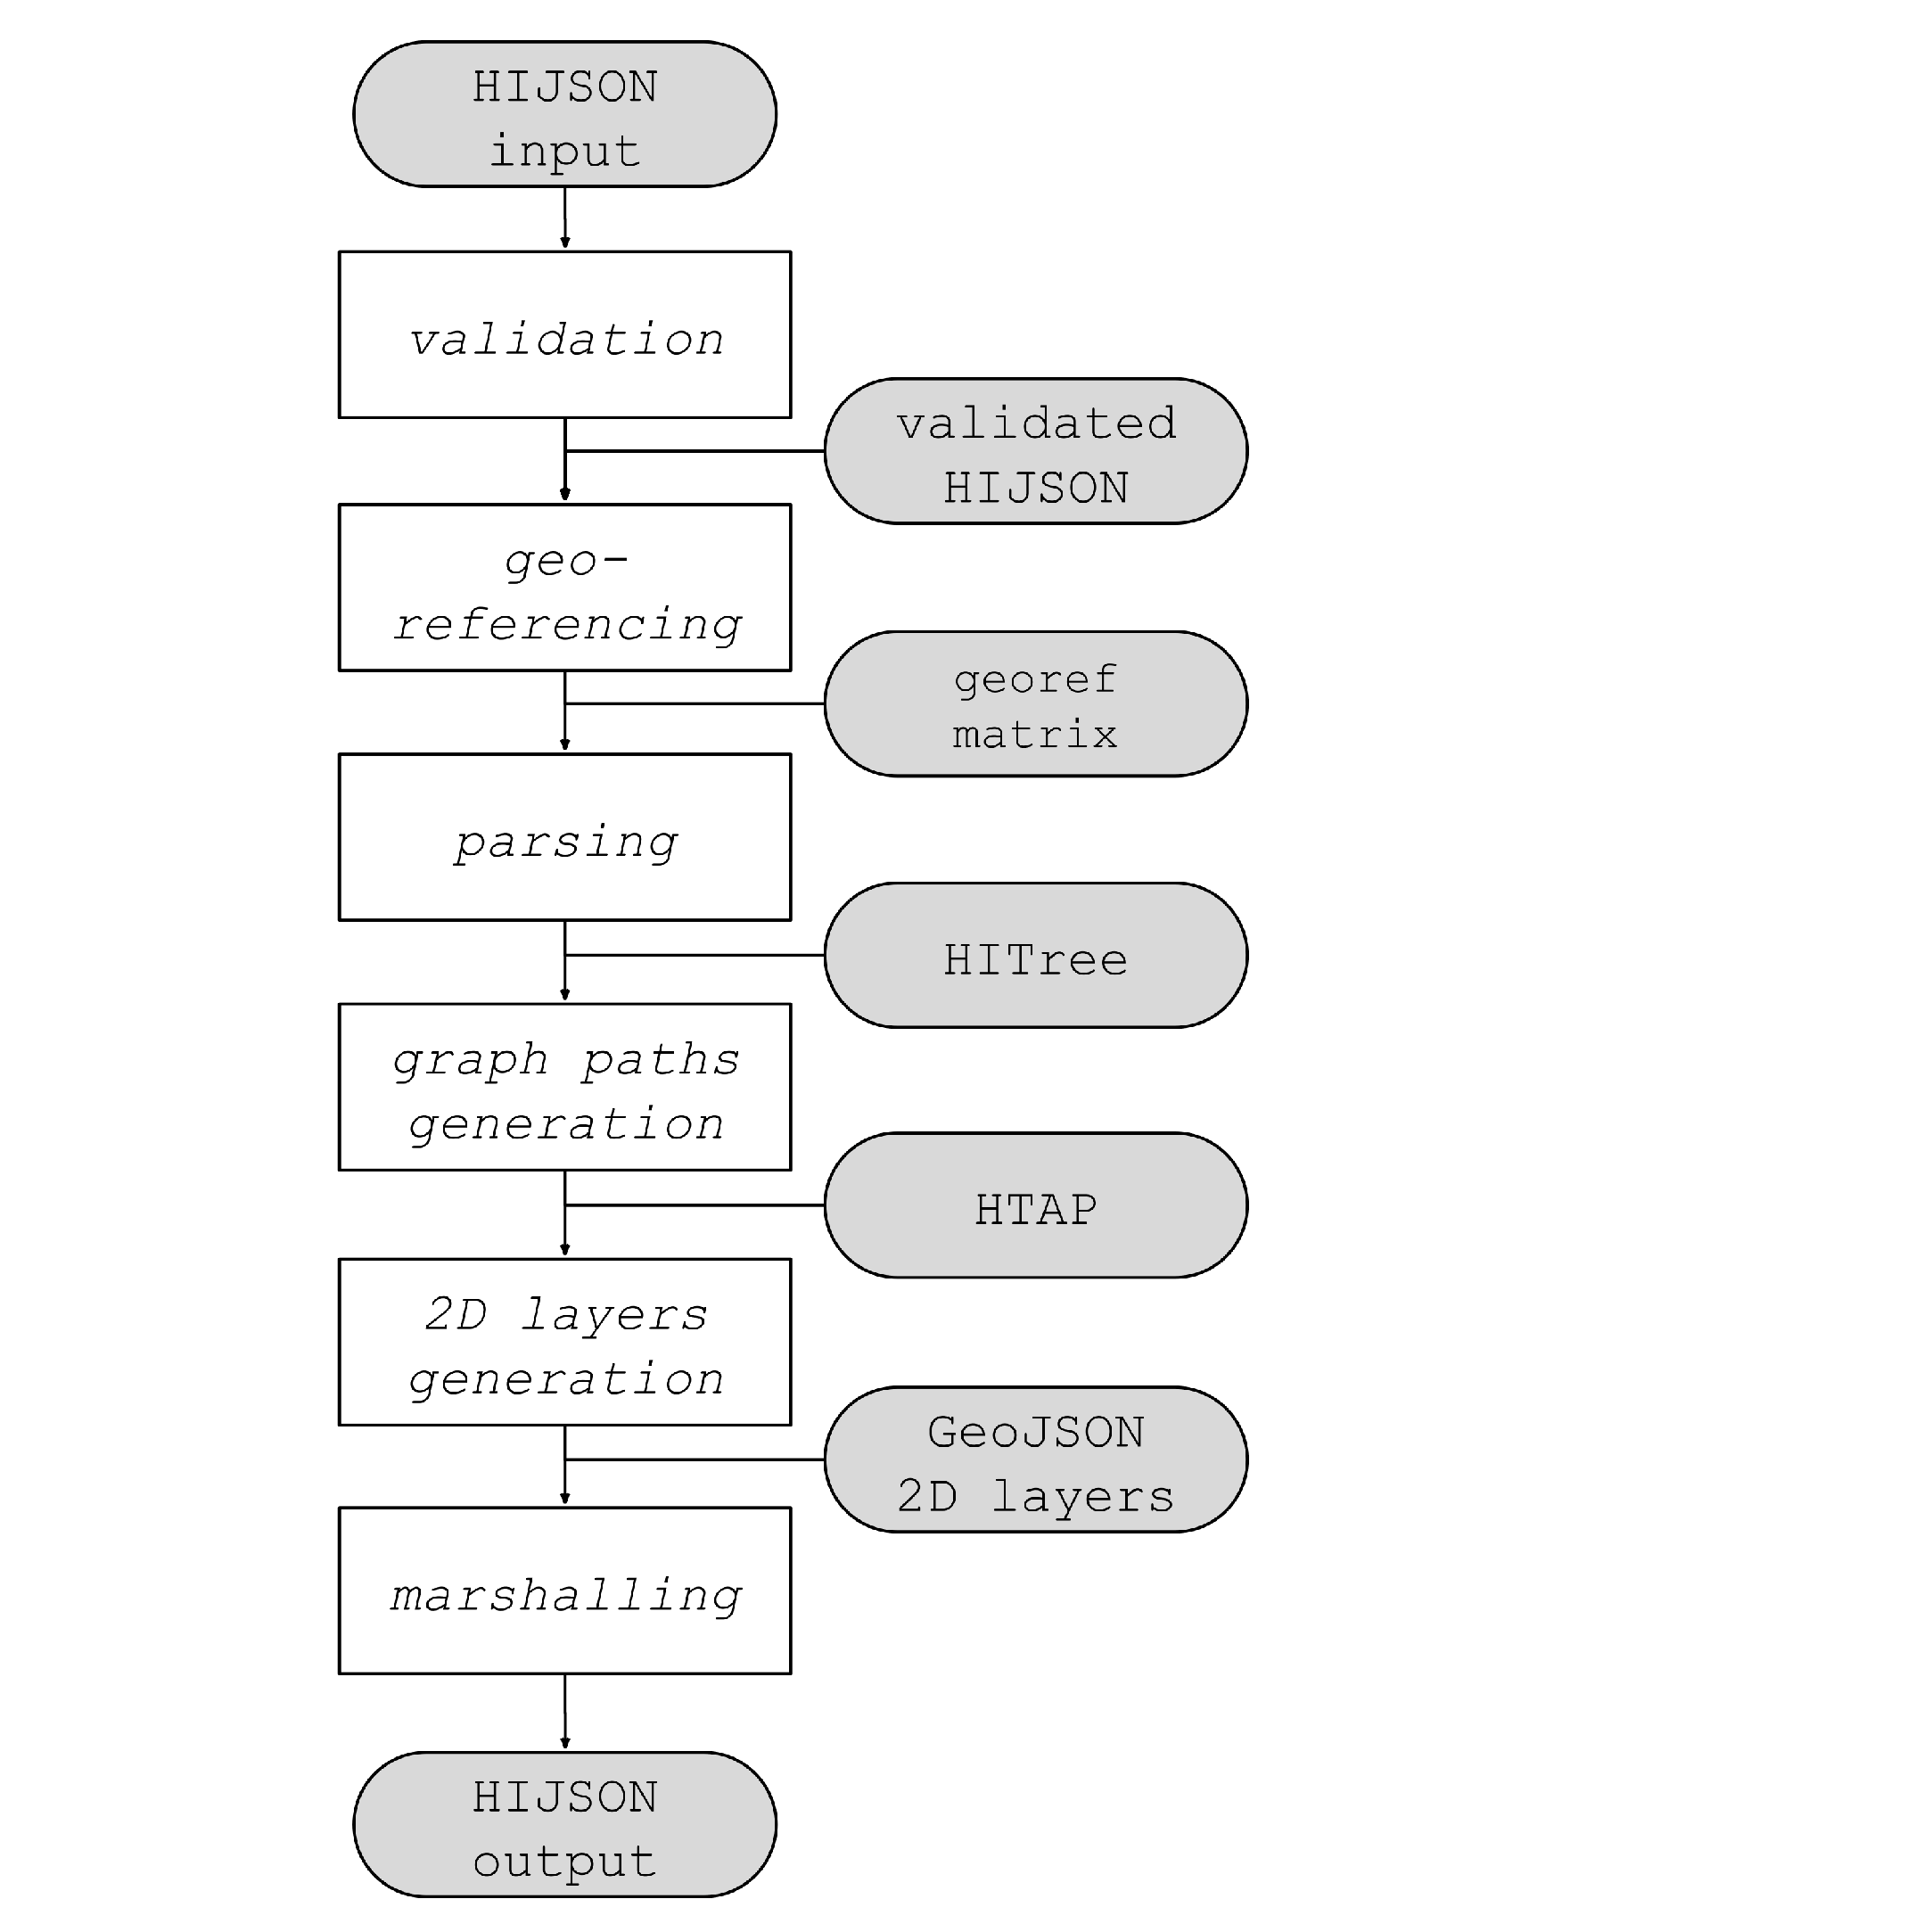
\epsfig{file=images/pipeline.eps, height=0.4\textwidth}
\caption{``HIJSON processing pipeline''}
\label{fig:pipeline}
\end{figure}

\begin{enumerate}
\def\labelenumi{\arabic{enumi}.}
\itemsep1pt\parskip0pt\parsep0pt
\item
  \textit{\texttt{validation}} - The first one is the validation stage. In
  order to begin with the effective transformations the input HIJSON
  document must be compliant with the rules defined in (AGGIUNGERE REF
  TO PARAGRAFO REGOLE DI VALIDITA'). In the case the validation stage
  fails, processing aborts and do not continue to following stages. If
  the stage success, the output for the next stage is a validated
  HIJSON.
\item
  \textit{\texttt{georeferencing}} - In the second stage, in order to allow
  for continuous outdoor/indoor navigation, the system needs to compute
  the georeferencing matrix, a linear operator able to transform local
  coordinates into global coordinates (referred to world coordinate
  system as latitude and longitude misures) and viceversa. This task is
  accomplished by solving a linear system obtained from information
  contained in HIJSON configuration part and precisely from the
  correnspondance of three real word points to three points included
  into the HIJSON document.
\item
  \textit{\texttt{parsing}} - The parsing stage, takes the validated and
  georeferenced HIJSON as its input, that as illustrated before can be
  thought of as a list of HIJSON Elments, parses them and produce an
  istance of HIJSON Tree. The HIJSON Tree is an object in memory
  representing the tree hierarchical structure of the building described
  by the HIJSON document.
\item
  \textit{\texttt{graph paths generation}} - The fourth stage is in charge
  of the generation of the graph paths. This aim is accomplished
  according to the algorithm described in (AGGIUNGERE RIFERIMENTO A
  \#\#\#\# Automatic generation of valid paths). The graph paths will be
  useful afterwards to coumpute valid paths from couple of point of
  interest on the graph. Once the graph paths has been computed, the
  input HIJSON Tree is augmented with paths information, becoming what
  has been called an HTAP (HIJSON Tree Augmented with Paths).
  Augmentation always takes place as leaf nodes added as children of a
  specific (e.g. ``room'') level.
\item
  \textit{\texttt{2D layers generation}} - The fifth stage is the
  generation of GeoJSON layer. For each level, the system generates one
  geoJSON layer that will be use for the creation of 2D map. Each layer
  contains the children of `level' node in the HIJSON Tree. Every class
  contains a boolean value that is used to choose which class will be a
  part of geoJSON layer. Every element has a geographical coordinates
  calculated by the transformation matrix with regard to the local
  coordinates of the HIJSON element.
\item
  \textit{\texttt{marshalling}} - The last stage is responsible of execute
  a serialization of the the transformed data. Tasks like breaking
  dependency-loops and stringification are performed. This stage is
  useful mainly serverside, as and the output is stored ready to be
  served to any requiring client.
\end{enumerate}

\subsubsection{Algorithmics: automatic generation of valid paths}\label{algorithmics-automatic-generation-of-valid-paths}

The fourth stage of the processing pipeline is responsible for the
generation of a graph of valid paths through the entire model
represented by the intput HIJSON document. The graph generated according
to the algorithm described in the following, although not optimal,
ensures a complete coverage of the surface while limiting the numebr of
generated nodes. Resulting graph is weigthed on the edges with nodes
distances and each node represents alternatively:

\begin{enumerate}
\def\labelenumi{\alph{enumi}.}
\itemsep1pt\parskip0pt\parsep0pt
\item
  standard path node, i.e.~a junction node or possibly an endpoint of a
  path;
\item
  connection node, used as subproblem composing element in the divide et
  impera approch adopted (as described below).
\item
  element nodes ie. HIJSON Element (whose HIJSON Class explicitly grants
  his presence in the graph), typically an endpoint of a path;
\end{enumerate}

Such a graph allows for directions calculations between any two given
nodes. Although different approaches have been explored \cite{6999103}, 
a very classical solution has been selected in this case, so directions 
are actually computed clientside applying the Dijkstra's shortes route 
algorithm on the graph. 

Taking advantage of the hierarchical structure of the HIJSON document,
and according to the divide et impera approach, the problem of the graph
paths generation is splitted in several sub-problems which consist in
the computation of the sub-graphs relative to each room, or more
generally ambience. The sub-graphs are then linked together through the
connection nodes (which in most cases represents doors). The resolution
of each sub-problem (as depicted in figure METTERE RIFERIMENTO ALLA
FIGURA), is composed by 4 phases:

\begin{enumerate}
\def\labelenumi{\arabic{enumi}.}
\itemsep1pt\parskip0pt\parsep0pt
\item
  Computation of the walkable area of the ambience: this task is
  accomplished subtracting area of the possibly encumbrances to the area
  of the ambience; the result is tipically a surface with holes;
\item
  Triangulation of the walkable area: the computed surface is
  triangulated taking into account the presence of holes;
\item
  Identification of graph nodes: for each triangle side completely
  internal to the area, its midpoint is selected as standard path node;
\item
  Junction of nodes: nodes relative to the same triangle are then linked
  together; both element nodes and connection nodes (i.e.~doors) are
  linked to the nearest node in the ambience (i.e.~room).
\end{enumerate}

\begin{figure*}[!htbp]
  \centering
  \begin{subfigure}[b]{0.235\textwidth}
    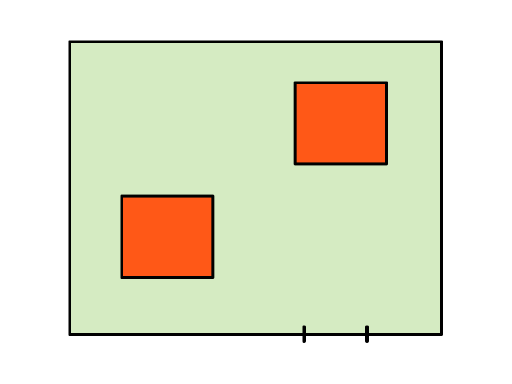
\includegraphics[width=\textwidth]{images/graph-generation/single/graph-generation-1}
    \caption{}
    \label{fig:graph-generation-a}
  \end{subfigure}
  ~
  \begin{subfigure}[b]{0.235\textwidth}
    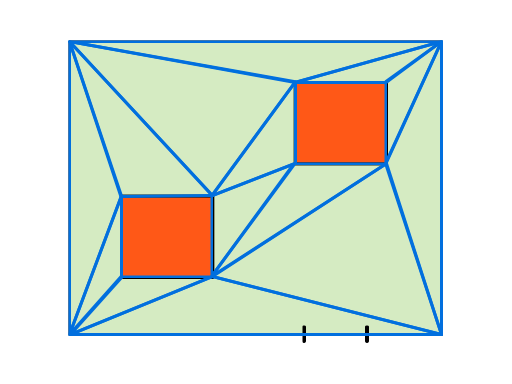
\includegraphics[width=\textwidth]{images/graph-generation/single/graph-generation-2}
    \caption{}
    \label{fig:graph-generation-b}
  \end{subfigure}
  ~
  \begin{subfigure}[b]{0.235\textwidth}
    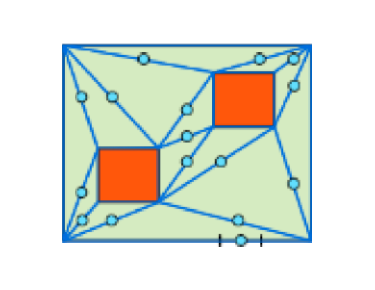
\includegraphics[width=\textwidth]{images/graph-generation/single/graph-generation-3}
    \caption{}
    \label{fig:graph-generation-c}
  \end{subfigure}
  ~
  \begin{subfigure}[b]{0.235\textwidth}
    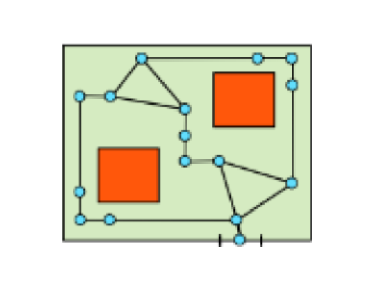
\includegraphics[width=\textwidth]{images/graph-generation/single/graph-generation-4}
    \caption{}
    \label{fig:graph-generation-d}
  \end{subfigure}
  
  \caption{Graph paths generation: 
    (a) detection of obstacles and computation of walkable area; 
    (b) triangulation of walkable area; 
    (c) identification of graph nodes area; 
    (d) junction of nodes.
  }
  \label{fig:graph-generation}
\end{figure*}

\subsection{HIJSON Class definition}\label{hijson-class-definition}

To exploit the possibilities offered by HIJSON Toolkit, along with the
HIJSON document, some custom dynamic behaviours must be described. These
behaviours encapsulate the specificities relative to comminucation
procols with the sensors as well as user interaction peculirities. The
interface for these behaviours is the HIJSON Class.

\begin{figure}[!h]
\centering
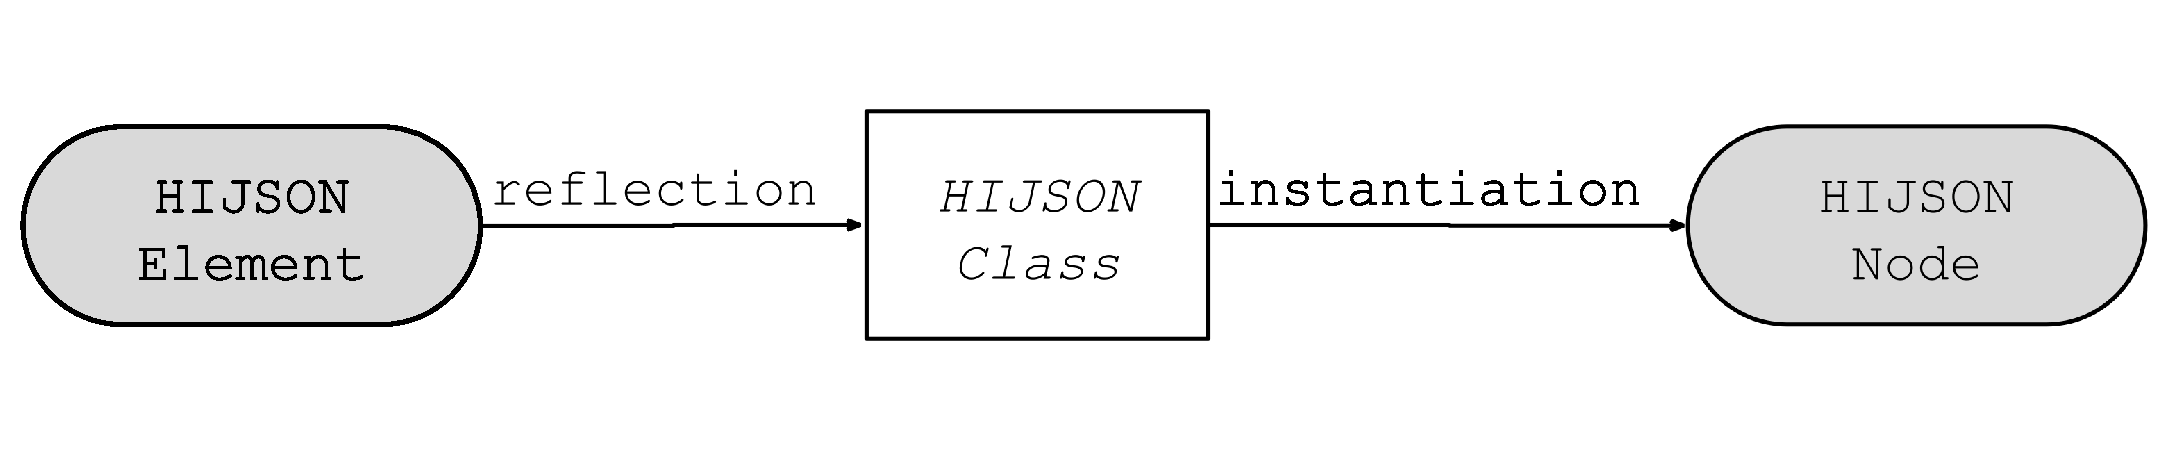
\epsfig{file=images/element-class-node.eps, width=0.44\textwidth}
\caption{``HIJSON Element/Class/Node relashionship''}
\label{fig:elem-class-node-rel}
\end{figure}

Each HIJSON Element of the HJSON document given as input, has a dynamic
counterpart, a running instance called HIJSON Node, instantiated
according to the corresponding HIJSON Class via relfection methods (see
picture XXXXX).

To specify a new HIJSON Class means to extend the Toolkit to deal with a
new class of HIJSON Element.

To extend the toolkit to deal with a new class of HIJSON Element is
required to to specify a new HIJSON Class, defining the following
properties and methods:

\begin{itemize}
\item
  \texttt{in\_graph}: a boolean value to express if the element is an
  approachable point in the graph paths;
\item
  \texttt{in\_2D\_map}: a boolean value to express if the element is
  wanted in the 2D map;
\item
  \texttt{get2DStyle}: a method that returns the 2D map appearence of
  the element, essentially HTML and CSS code;
\item
  \texttt{get3DModel}: a method that returns the 3D model appearence of
  the element, a \emph{THREE.js Object3D};
\item
  \texttt{getWidget}: a method that returns the information widget, a
  \emph{React} component;
\item
  \texttt{getProxy}: a method that returns server side proxy which
  encapsulate IoT sensor communication protocol, a \emph{Node.js
  module}.
\end{itemize}

User's needs for new indoor elements, different sensor equipment,
alternative representation on 2D or 3D viewport are accepted by the
definition of new HIJSON Classes that allows in this way single point
custom extension of the Toolkit capabilities.

\section{HJSON Web Framework}\label{hjson-web-framework}

The HJSON Web Framework responds to the needs of an extendable,
customizable, and scalable framework which provides at the same time IoT
monitoring, realtime multi-person tracking and crossfloor user
navigation.

Expandability and customizability derives from both design choises and
HIJSON inherent characteristics, the possibility of semantic extensions.
Scalablility is directly borrowed from technologies used for the
software development: \emph{JavaScript} language, using \emph{Node.js},
in particular \emph{Express.js} as backend framework, exploiting the
power of WebSocket protocol through the \emph{Socket.io} library.

Being supported by the web as bearing platform, the framework exposes
also an highly availability: it is so simple to use as to visit a
website, both from desktop or mobile devices, without explicit
requirements to install any software from proprietary stores (access to
which is often denied from business devices).

The HIJSON Web Framework deeply relies on HIJSON Toolkit and offers the
overal client/server architecture and a convinient, highly intractive
user interface, leaving aside the specific indoor positioning system and
the IoT sensors, to deal with a robust interface is provided and
described in the following seciton.

\subsection{Applications}\label{applications}

\begin{figure*}[!hb]
\centering
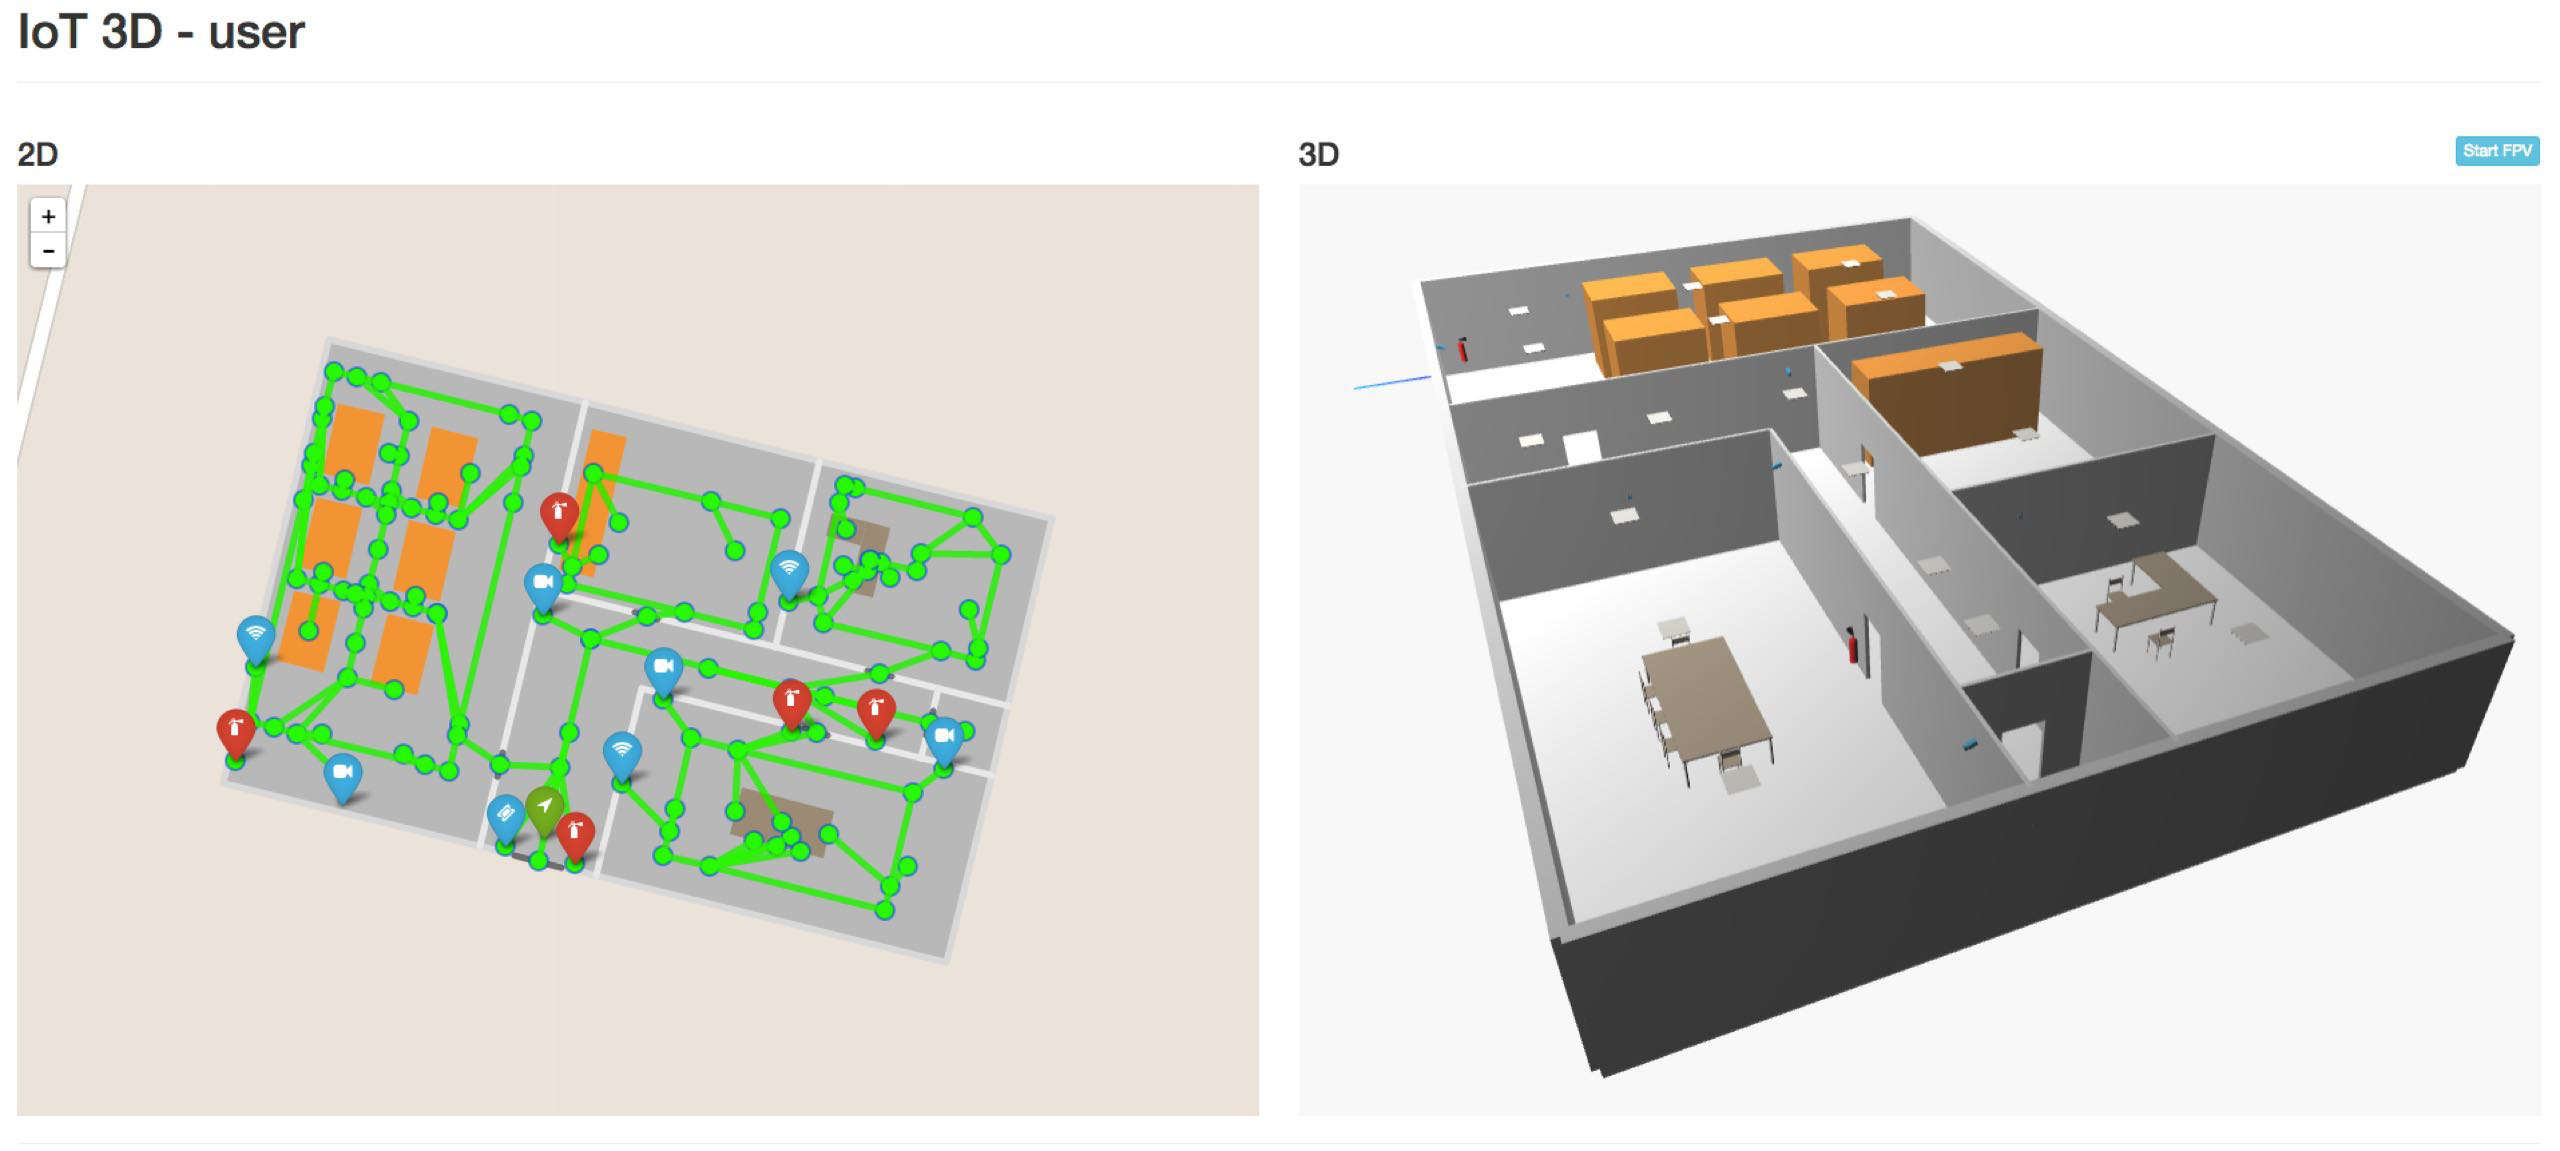
\includegraphics[width=\textwidth]{images/web-framework.png}
\caption{``HIJSON Web Framework UI''}
\label{fig:web-framework-ui}
\end{figure*}

The Framework has been designed focus on two different possible kind of
users: the \emph{Explorer} and the \emph{Supervisor}. They have
different requirements and are likely equipped with different devices:
while the \emph{Supervisor} monitors the indoor environment through a
desktop workstation, the \emph{Explorer} has a smartphone available and
needs to be routed across the building.

\subsubsection{IoT monitoring}\label{iot-monitoring}

Every element in the HIJSON environment is capable of showing information
about itself,  so it can be analyzed by the user. The modularity of the HIJSON
Toolkit permits to show  particular information or UI about a specific object,
using polymorphic behaviours of the different HIJSON Nodes. If an object is
connected to the network and it is capable of interaction, the user can
benefit of its functions through the system (e.g. if the object is a
thermostat, the user can see the temperature in the room and can turn on/off
the heating). If the object isn't interactive, the system can show static
information (e.g. for fire Extinguisher, the system shows the last date of
checking).

\subsubsection{Realtime multi-person tracking}\label{realtime-multi-person-tracking}

A typical task performed by a \emph{Supervisor} can be the monitoring of users
locations  inside the building. This operation can be required for various
reasons, e.g. security or  logistics. The devices that equips the
\emph{Explorers} can be used to track their position  in realtime, giving the
\emph{Supervisors} the whole picture of the presences inside the  building in
every moment.

--- da controllare cosa tenere rispetto a quanto già scritto dopo ---

The system can be used for access monitoring. On 2D map will be a marker
for each person in the building, whereas on the 3D model will be a 3D
model of user. With an appropriate system of indoor localization, every
person sends its position in real time. The 2D map and the 3D model is
automatically refreshed. The user can ask for information about person,
in function of the use of the system.

The communication of the current position happens with the socket.io
library. Every user sends an object like this:

\begin{verbatim}
currentPosition = {
    coordinates: [x, y],
    levelId: level-ID  
}
\end{verbatim}

For every change of the coordinates or level, an \emph{emit} event will
be generated, according to the socket.io library, which sends to the
server the new current position. The server sends to the connected
client the updated current position of the users connected. In the
client-side, when the \emph{on} event of socket.io library is hit, there
will be a refresh of the marker in 2D map and the 3D model in the 3D
representation. With Observer pattern implemented in socket.io library,
it is possibile to have a realtime multi-person tracking. This system
permits to be indipendent from the tool that gets the position of the
users: the only requisite is to send the position like the object
described above.

--- fine controllo ---

\subsubsection{Crossfloor user navigation}\label{crossfloor-user-navigation}

As shown in the algorithmics section, the HIJSON Toolkit provides a particular
strategy  to assemlbe a graph of possible paths inside the building. This
graph, represented also  in the form of a weighted adjacency matrix, can be
easely used to compute paths between  two nodes inside the building. To
achieve this result, the matrix, which edges are weighted  according to the
distance between two nodes, is used as input in an applicaiton of the
Dijkstra's algorithm. The result is the shortest path between two selected
nodes of the graph.  Thanks to the crossfloor connections of nodes
representing stairs or elevators, the paths  calculated can also start and end
on different stories.

\subsection{Architecture}\label{architecture}

Like the vast majority of the web based application, the Framework exposes an
overall architecture that is inherently \emph{client/server}. In particular,
two different type of possible client are identifiable: the \emph{Supervisor}
client and the \emph{Explorer} client. Both of them connect to the same
server.

The indoor space described by the HIJSON document provided as input is
processed by the server (cfr. PROCESSING PIPELINE). After that any connecting
\emph{Explorer} client, presumably through a mobile device, will be provided
with the information to perform crossfloor navigation of the building, while
reporting user position to the server. The server will feed any connecting
\emph{Supervisor} client with users positions, along with data from sensor-
equipped things present in the environment, realizing the IoT monitoring and
the realtime multi-person tracking.

\begin{figure*}[t]
\centering
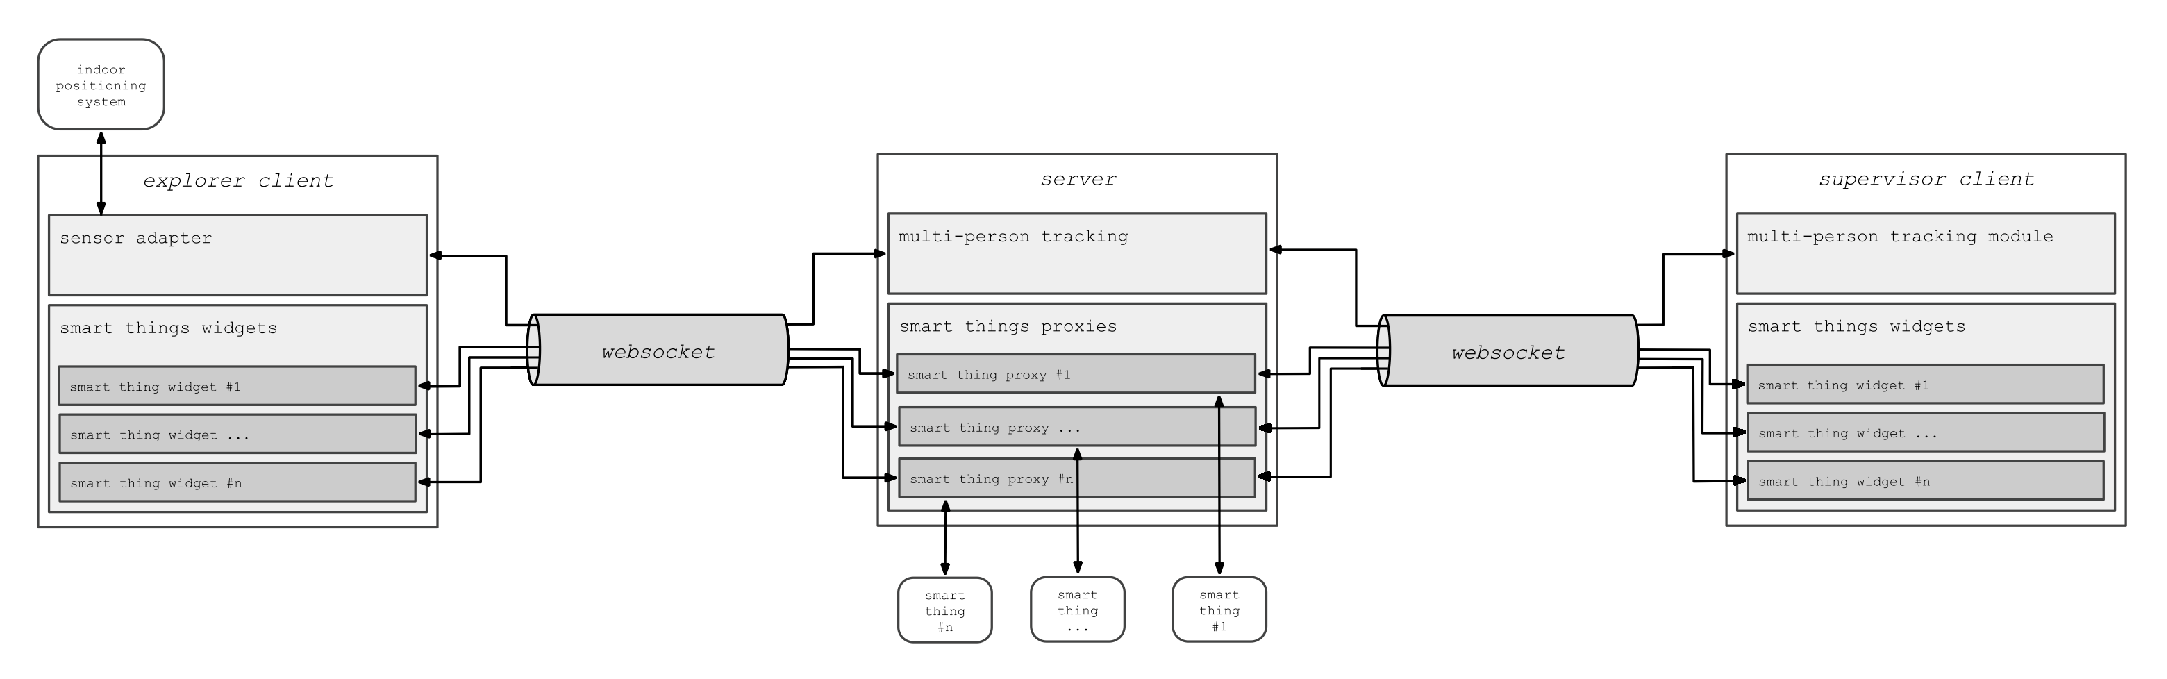
\epsfig{file=images/architecture.eps, width=\textwidth}
\caption{``HIJSON Web Toolkit architecture''}
\label{fig:pipeline}
\end{figure*}

\subsubsection{Server Architecture}\label{server-architecture}

The architecture of the server is depicted in XXXX. A web server module
is responsible for listenning to connecting clients. Each client
connection is handled by the web server module providing all the
required resources and opening one websocket channel, through which will
flow \emph{Explorer} and/or \emph{Supervisor} communication protocol
data. In particular, \texttt{multi-person\ tracking} module receives
position data from \emph{Explorer} clients. It aggregates and sends
these information to connected \emph{Supervisor} clients through the
websocket channel, using a simple but realible protocol later described.
Indipendence from particular IoT sensor equipment communication protocol
is achieved by the \texttt{smart\ things\ proxies} module through the
proxies modules obtained by the HIJSON Class definition
(\texttt{getProxy} method previuosly described).

\subsubsection{Explorer client architecture}\label{explorer-client-architecture}

The \emph{Explorer} client architecture is generally deployed on a
mobile device, usually supplied to a user who needs to be routed across
the environment described by HIJSON document. The
\texttt{sensor\ adapter} module encapsulates the communication logic
with the indoor positioning system. The presence of this module ensures
indipendece from particularly tecnology allowing client \emph{Explorer}
to rely on different indoor positioning systems: INDICARE ESEMPI SENSATI
E CUTTING EDGE DI POSIZIONAMENTO INDOOR. INTRODURRE IL PROBLEMA DELLA
COMUNICAZIONE A LIVELLO API DEL BROWSER CON SENSORISTICA PER LA
RILEVAZIONE DELLA POSIZIONE.

Every time the \texttt{sensor\ adapter} observe a perceptible
modification in user position sends the new position information to the
server through the single opened websocket, using the a message with the
following syntax:

\begin{verbatim}
currentPosition = {
    coordinates: [x, y],
    levelId: level-ID  
}
\end{verbatim}

Relevant information includes, beside current coordinates, the
indication of the story of the possibly multilevel building the user is
in. The \texttt{smart\ things\ widgets} module being in common with the
client \emph{Supervisor}, has been treated in the next section.

\subsubsection{Supervisor client architecture}\label{supervisor-client-architecture}

The Client \emph{Supervisor} architecture shows two modules. The first
one, the \texttt{multi-person\ tracking} module, is responsible to
receive through the websocket, from the server information about
explorers of the environment, showing them in the user interface. The
second module, the \texttt{smart\ things\ widget} communicates with the
server to propose to the user realtime information about sensor-equipped
objects in the environment. Data passes through the single websocket
opened between the server and every \emph{Supervisor} Client. Rely on a
naive but effective communication protocol, each smart thing widget
exchaange data only with respective smart thing proxy on the server. To
ensure the the data is sent only when the user requires the information
relative to a specific smart thing, a widget lifecycle protocol is
implemented: it is based on the 4 events \texttt{on\_before\_show},
\texttt{on\_show}, \texttt{on\_before\_hide}, \texttt{on\_hide}
triggered, as suggested by their names when a widget is shown or hidden.
When the user requires information about a smart thing, its widget has
to be rendered, but \texttt{on\_before\_show} the server is notified to
connect via relative proxy to the sensor. Once connected, the server
begin to send data via webscocket. Received data is shown through the
wodget to the user. When done, or \texttt{on\_before\_hide} event of the
widget, a notification is sent to the server announcing to stop sending
data and the proxy close the connection to the sensor. Widget lifecycle
protocol ensures that only requiring data is sent from th eserver to the
client.

\section{Conclusions}\label{conclusions}

We presented HIJSON a GeoJSON extension for indoor mapping TRA GLI
SVILUPPI FUTURI: - GENERAZIONE GRAFICA IN AMBIENTE CAD DEL DOCUMENTO
HIJSON

REPOSITORY PUBBLICO DI ESTENSIONI SEMANTICHE: POTREBBE MAPPARE TUTTE
GLI SMART OBJECT CON CONTRIBUTI DALLA COMUNITÀ. 

%
% The following two commands are all you need in the
% initial runs of your .tex file to
% produce the bibliography for the citations in your paper.
\bibliographystyle{abbrv}
\bibliography{doceng2015}  % doceng2015.bib is the name of the Bibliography in this case
% You must have a proper ".bib" file
%  and remember to run:
% latex bibtex latex latex
% to resolve all references
%
% ACM needs 'a single self-contained file'!
%
%\balancecolumns
\end{document}
